%!TEX root = ../thesis.tex

\chapter{深对流对臭氧垂直分布的影响}

由第\ref{sec:effects_on_nox_profile}章分析可知,云切片算法得到的不同高度对流云内NO$_2$平均浓度,
可用于分析LNO$_2$和污染NO$_2$的地理分布并校验MERRA2-GMI的模拟结果。
由于LNO$_x$和对流输送可共同对O$_3$的垂直分布产生影响,因此本章利用同样的云切片方法得到云间的O$_3$平均浓度,
并分析输送和化学过程对其的贡献。

本章余下部分按照以下方式组织:
\ref{sec:model_settings_assimilation}节介绍WRF-Chem模式使用的闪电同化方案;
\ref{sec:o3_profile}节将O$_3$探空与WRF-Chem模式结果进行对比,并利用云切片方法计算1$^{\circ}$ $\times$ 1$^{\circ}$ 网格内不同高度的O$_3$平均浓度和MLS观测的O$_3$廓线与MERRA2-GMI模拟的O$_3$廓线进行对比分析;
\ref{sec:convec_impacts}节利用MERRA2-GMI和WRF-Chem的趋势诊断量分析动力输送和化学过程对O$_3$浓度变化的贡献;
\ref{sec:lnox_effects}节通过WRF-Chem的敏感性试验探讨了LNO$_x$在对流不同阶段对O$_3$垂直分布的影响;
最后是本章小结。


\section{模式设置} \label{sec:model_settings_assimilation}

本章第\ref{sec:o3_profile}节和\ref{sec:convec_impacts}节中的全球模拟设置与第\ref{sec:model_settings_gmi}节相同。
本章第\ref{sec:lnox_effects}节中的中国东南部模拟设置与第\ref{sec:model_settings_china}节相同。
由于中国东南部的对流生命期短,我们采用了闪电同化并利用晴空条件下的O$_3$探空资料修正了O$_3$的初始场,然后将模拟结果与探空和雷达对比。

闪电数据同化方法详见\citet{Fierro.2012}和\citet{Li.2017b},主要步骤为在发生闪电所处网格的垂直恒温层间,增加水汽质量混合比。

\begin{equation} \label{eq:lda}
Q_{v}=A Q_{\mathrm{sat}}+B Q_{\mathrm{sat}} \tanh (C X)\left[1-\tanh \left(D Q_{g}^{\alpha}\right)\right]
\end{equation}

式(\ref{eq:lda})中,Q$_{sat}$ 为水汽饱和混合比(g kg$^{−1}$),Q$_g$为霰粒混合比(g kg$^{−1}$),X 为闪电频率。
本研究选择263.15 和 290.15 K作为恒温层的上下界限,其目的是为了让对流在行星边界层中快速扎根,因为对流层低层的Q$_v$更深\citep{Marchand.2014,Finney.2016,Li.2017b}。
参数设置参考\citet{Li.2017b}:A=0.94,B=0.2,C=0.001,D=0.25,α=2.2。
其中网格化的总闪数据通过WRF的辅助输入流进行每10分钟的读取。
例如,如果闪电同化开始于05:00 UTC,时间步长为10 min,则将05:00--05:10 UTC之间特定网格中所有闪电数相加作为此期间的贡献。
在下一个时间步长,闪电被归类为下一个新组。
因此,闪电数即闪电频率的密度(单位:flash每10 min 每dx km 每dy km),其中dx和dy分别是模型网格在x和y方向的分辨率。
如\citet{Fierro.2012}和\citet{Li.2017b}所述,这可以确保所有嵌套层中的闪电密度相同。
此外,闪电数也被直接同化进WRF-Chem中,该方法已被应用于社区多尺度空气质量(CMAQ,\citet{Kang.2019,Kang.2019a,Kang.2020}模式中。

与雷达观测相比,2019年7月25日和2020年9月1日模拟的对流初生时间,较实际情况分别提前了60分钟和30分钟(图\ref{fig:comp_crf_2019}和图\ref{fig:comp_crf_2020}),闪电数据也以相同的时间间隔提前同化。
对于下文的结果比较,我们选择匹配的阶段而不是相同的时间。

2019年7月25日的热对流在初始时呈现为孤立的热泡,WRF-Chem再现了初始阶段孤立对流的位置和强度(图\ref{fig:comp_crf_2019}a和\ref{fig:comp_crf_2020}d)。
在05:40 UTC时,对流系统呈现东北-西南向,最大组合雷达反射率达到60 dBZ(图\ref{fig:comp_crf_2019}b),强度大于模拟的对流(最大组合雷达反射率为55 dBZ,图\ref{fig:comp_crf_2019}e)。
将模拟的对流核心区的雷达反射率垂直剖面与观测结果进行比较(图\ref{fig:comp_dbzcross_2019}),
虽然对流与雷达距离过远造成缺失数据较多,但是在未进行人工插值的条件下,孤立对流的水平和垂直结构仍大致显示。
模拟的45 dBZ等值线达到12 km,但由于10 km 以上的数据质量低,观测到的等值线仅达到10 km。

2020年9月1日观测到的飑线在北部初生,然后加强,并向观测点移动(图\ref{fig:comp_crf_2020})。
对流旺盛阶段(最大组合雷达反射率为60 dBZ)大致在05:50 UTC,与TROPOMI过境时间相符(图\ref{fig:comp_dbzcross_2020}b和e)。
虽然该飙线抵达的最高高度低于2019年的热对流,但对流层低层(2--8 km)的反射率更大更广(图\ref{fig:comp_dbzcross_2020})。
由于模拟的对流消散区偏离了雷达观测到的消散区,这导致与臭氧探空仪比较的区域设置在站点的西侧(图\ref{fig:comp_dbzcross_2020}c和f)。


\begin{figure}[!htbp]
\centering
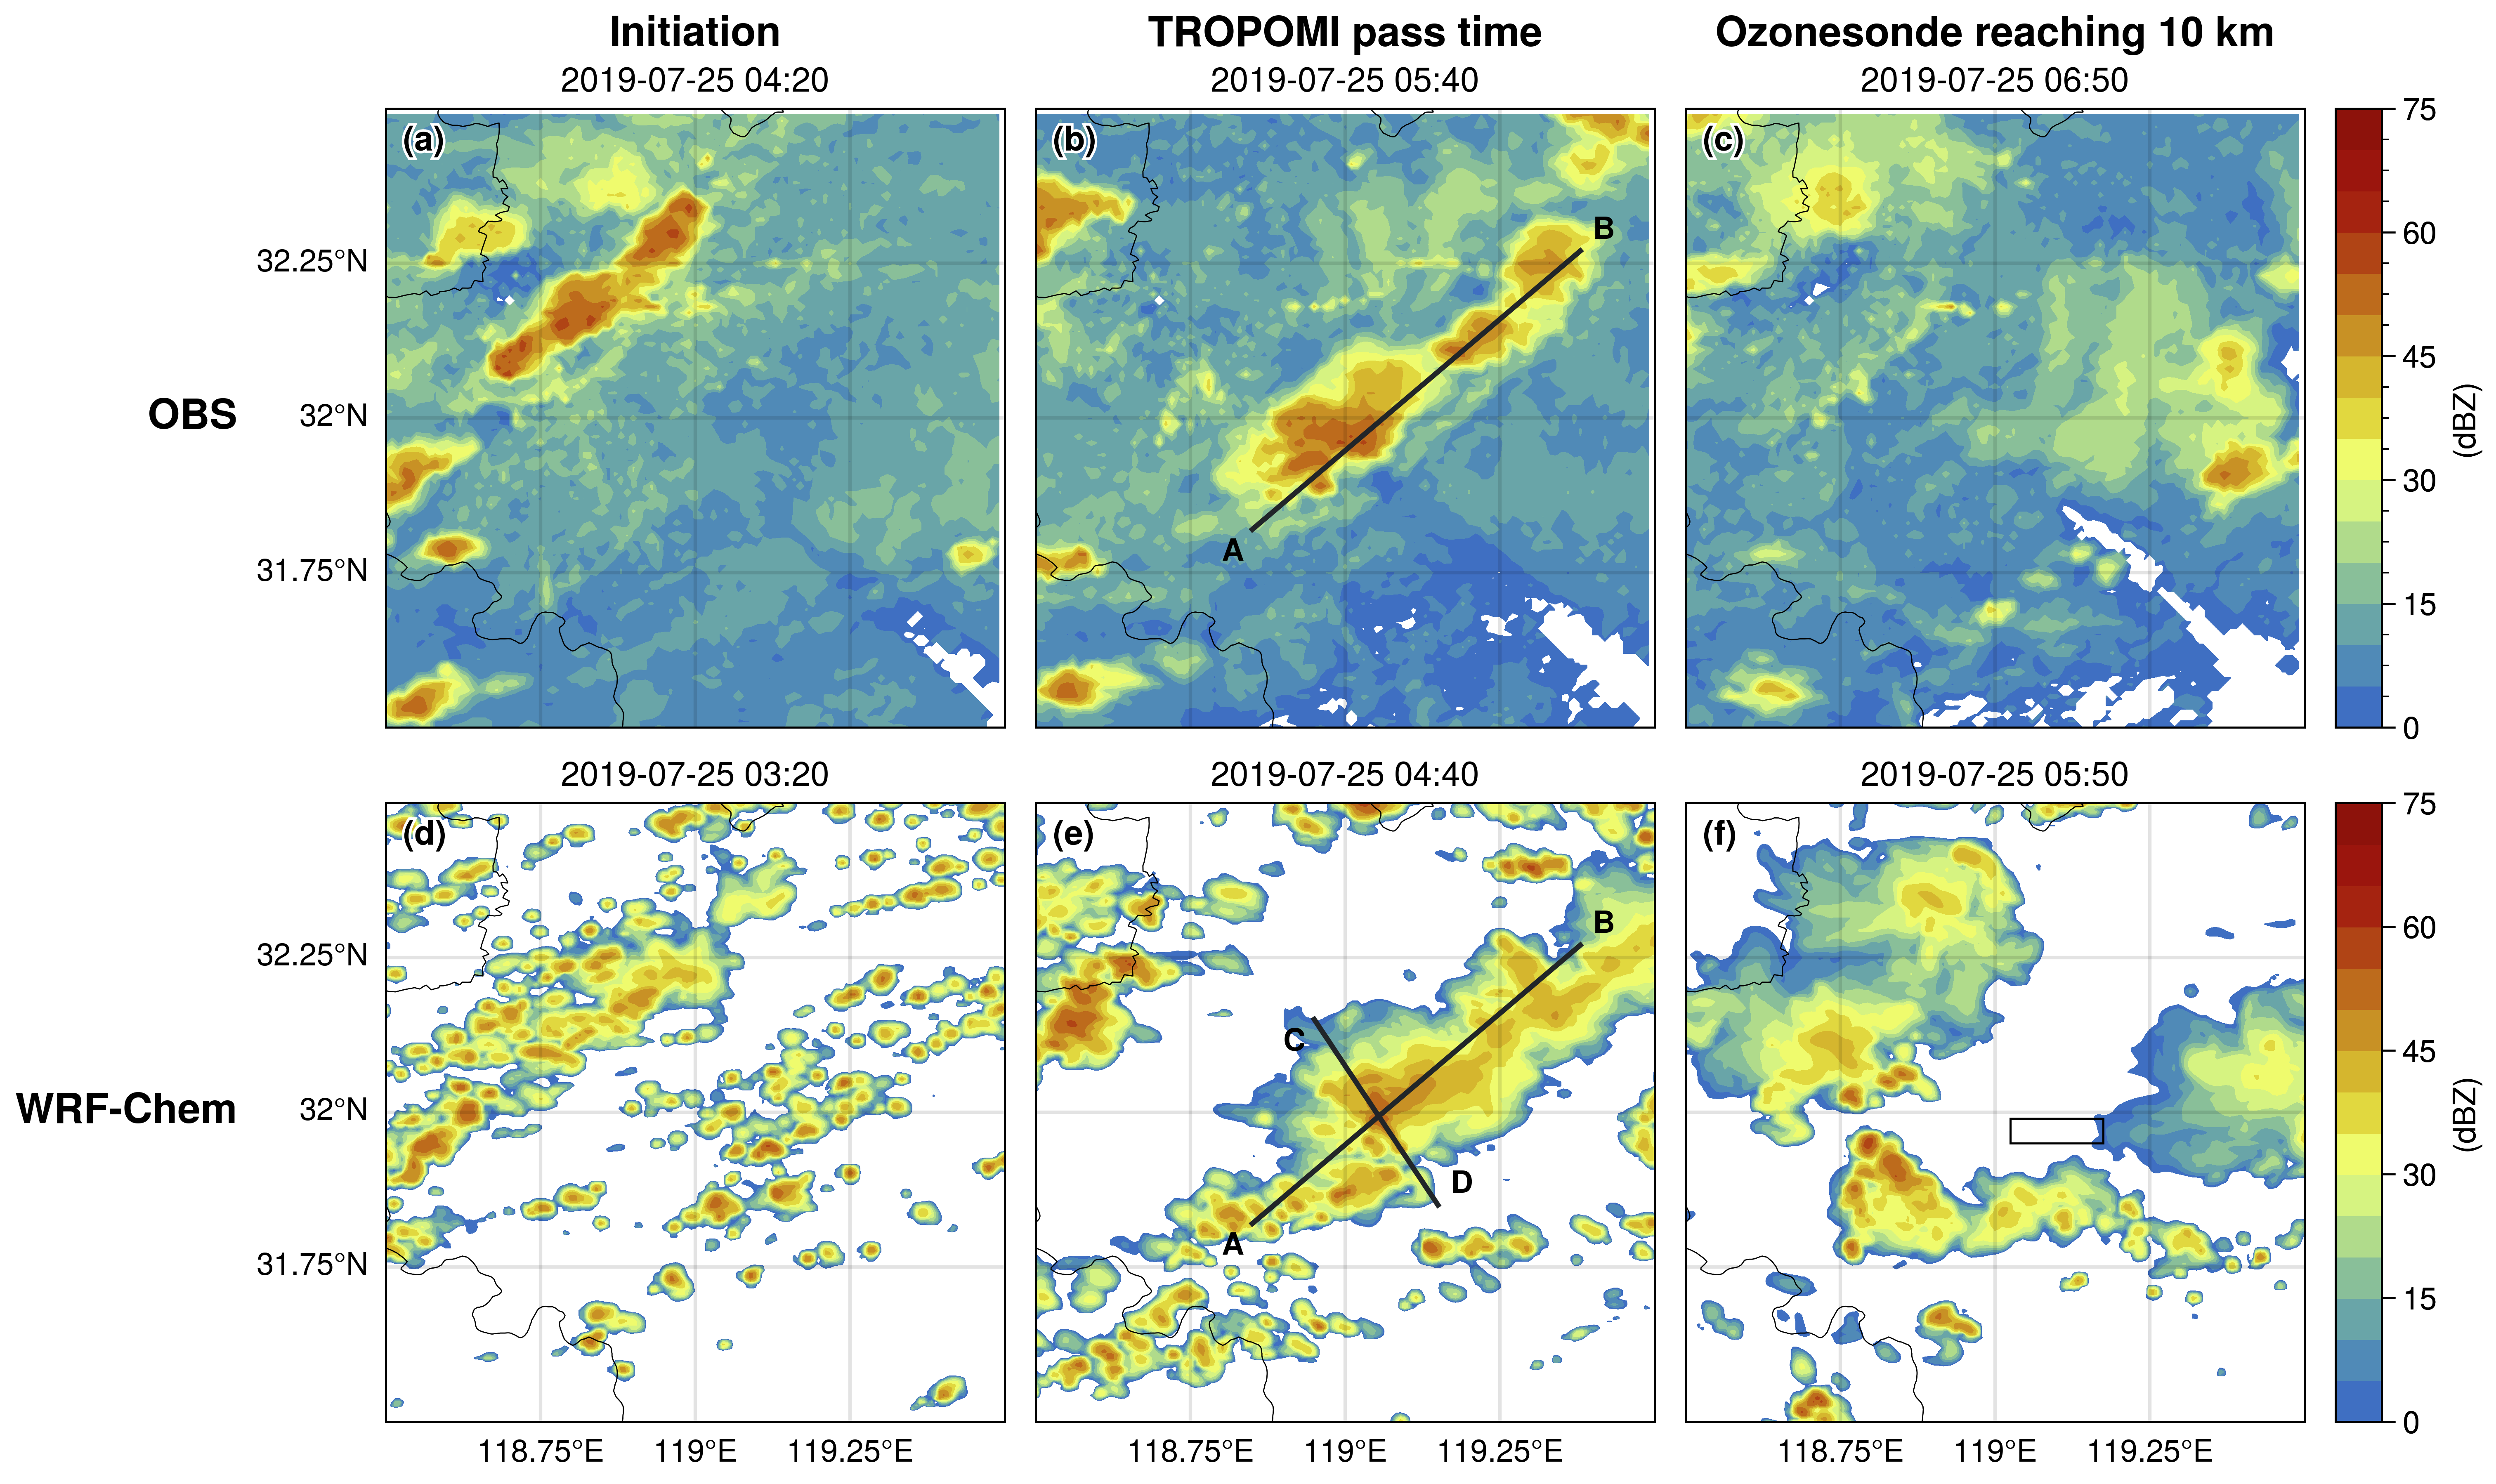
\includegraphics[width=0.9\textwidth]{./figures/comp_crf_2019.png}
\caption{在 (a) 04:20 UTC、(b) 05:40 UTC 和 (c) 06:50 UTC 观测到的雷达组合反射率。
         (d--e) WRF-Chem 在雷达观测时间前一小时模拟的雷达组合反射率。
         (b) 和 (e) 中的 AB 实线是图 \ref{fig:comp_dbzcross_2019} 的剖面线。
         (e)中的CD实线是图\ref{fig:tendency_o3}b的剖面线。
         黑色矩形是与臭氧探空仪进行比较的区域。\\
         Figure \ref{fig:comp_crf_2019}. Observed radar composite reflectivity at (a) 04:20 UTC, (b) 05:40 UTC, and (c) 06:50 UTC.
        (d--e) WRF-Chem simulated composite reflectivity one hour before the radar observation times.
        The AB solid lines in (b) and (e) are cross section lines for Fig. \ref{fig:comp_dbzcross_2019}.
        The CD solid line in (e) is the cross section line for Fig. \ref{fig:tendency_o3}b.
        The black rectangle is the region for the comparison with ozonesonde.}
\label{fig:comp_crf_2019}
\end{figure}

\begin{figure}[!htbp]
\centering
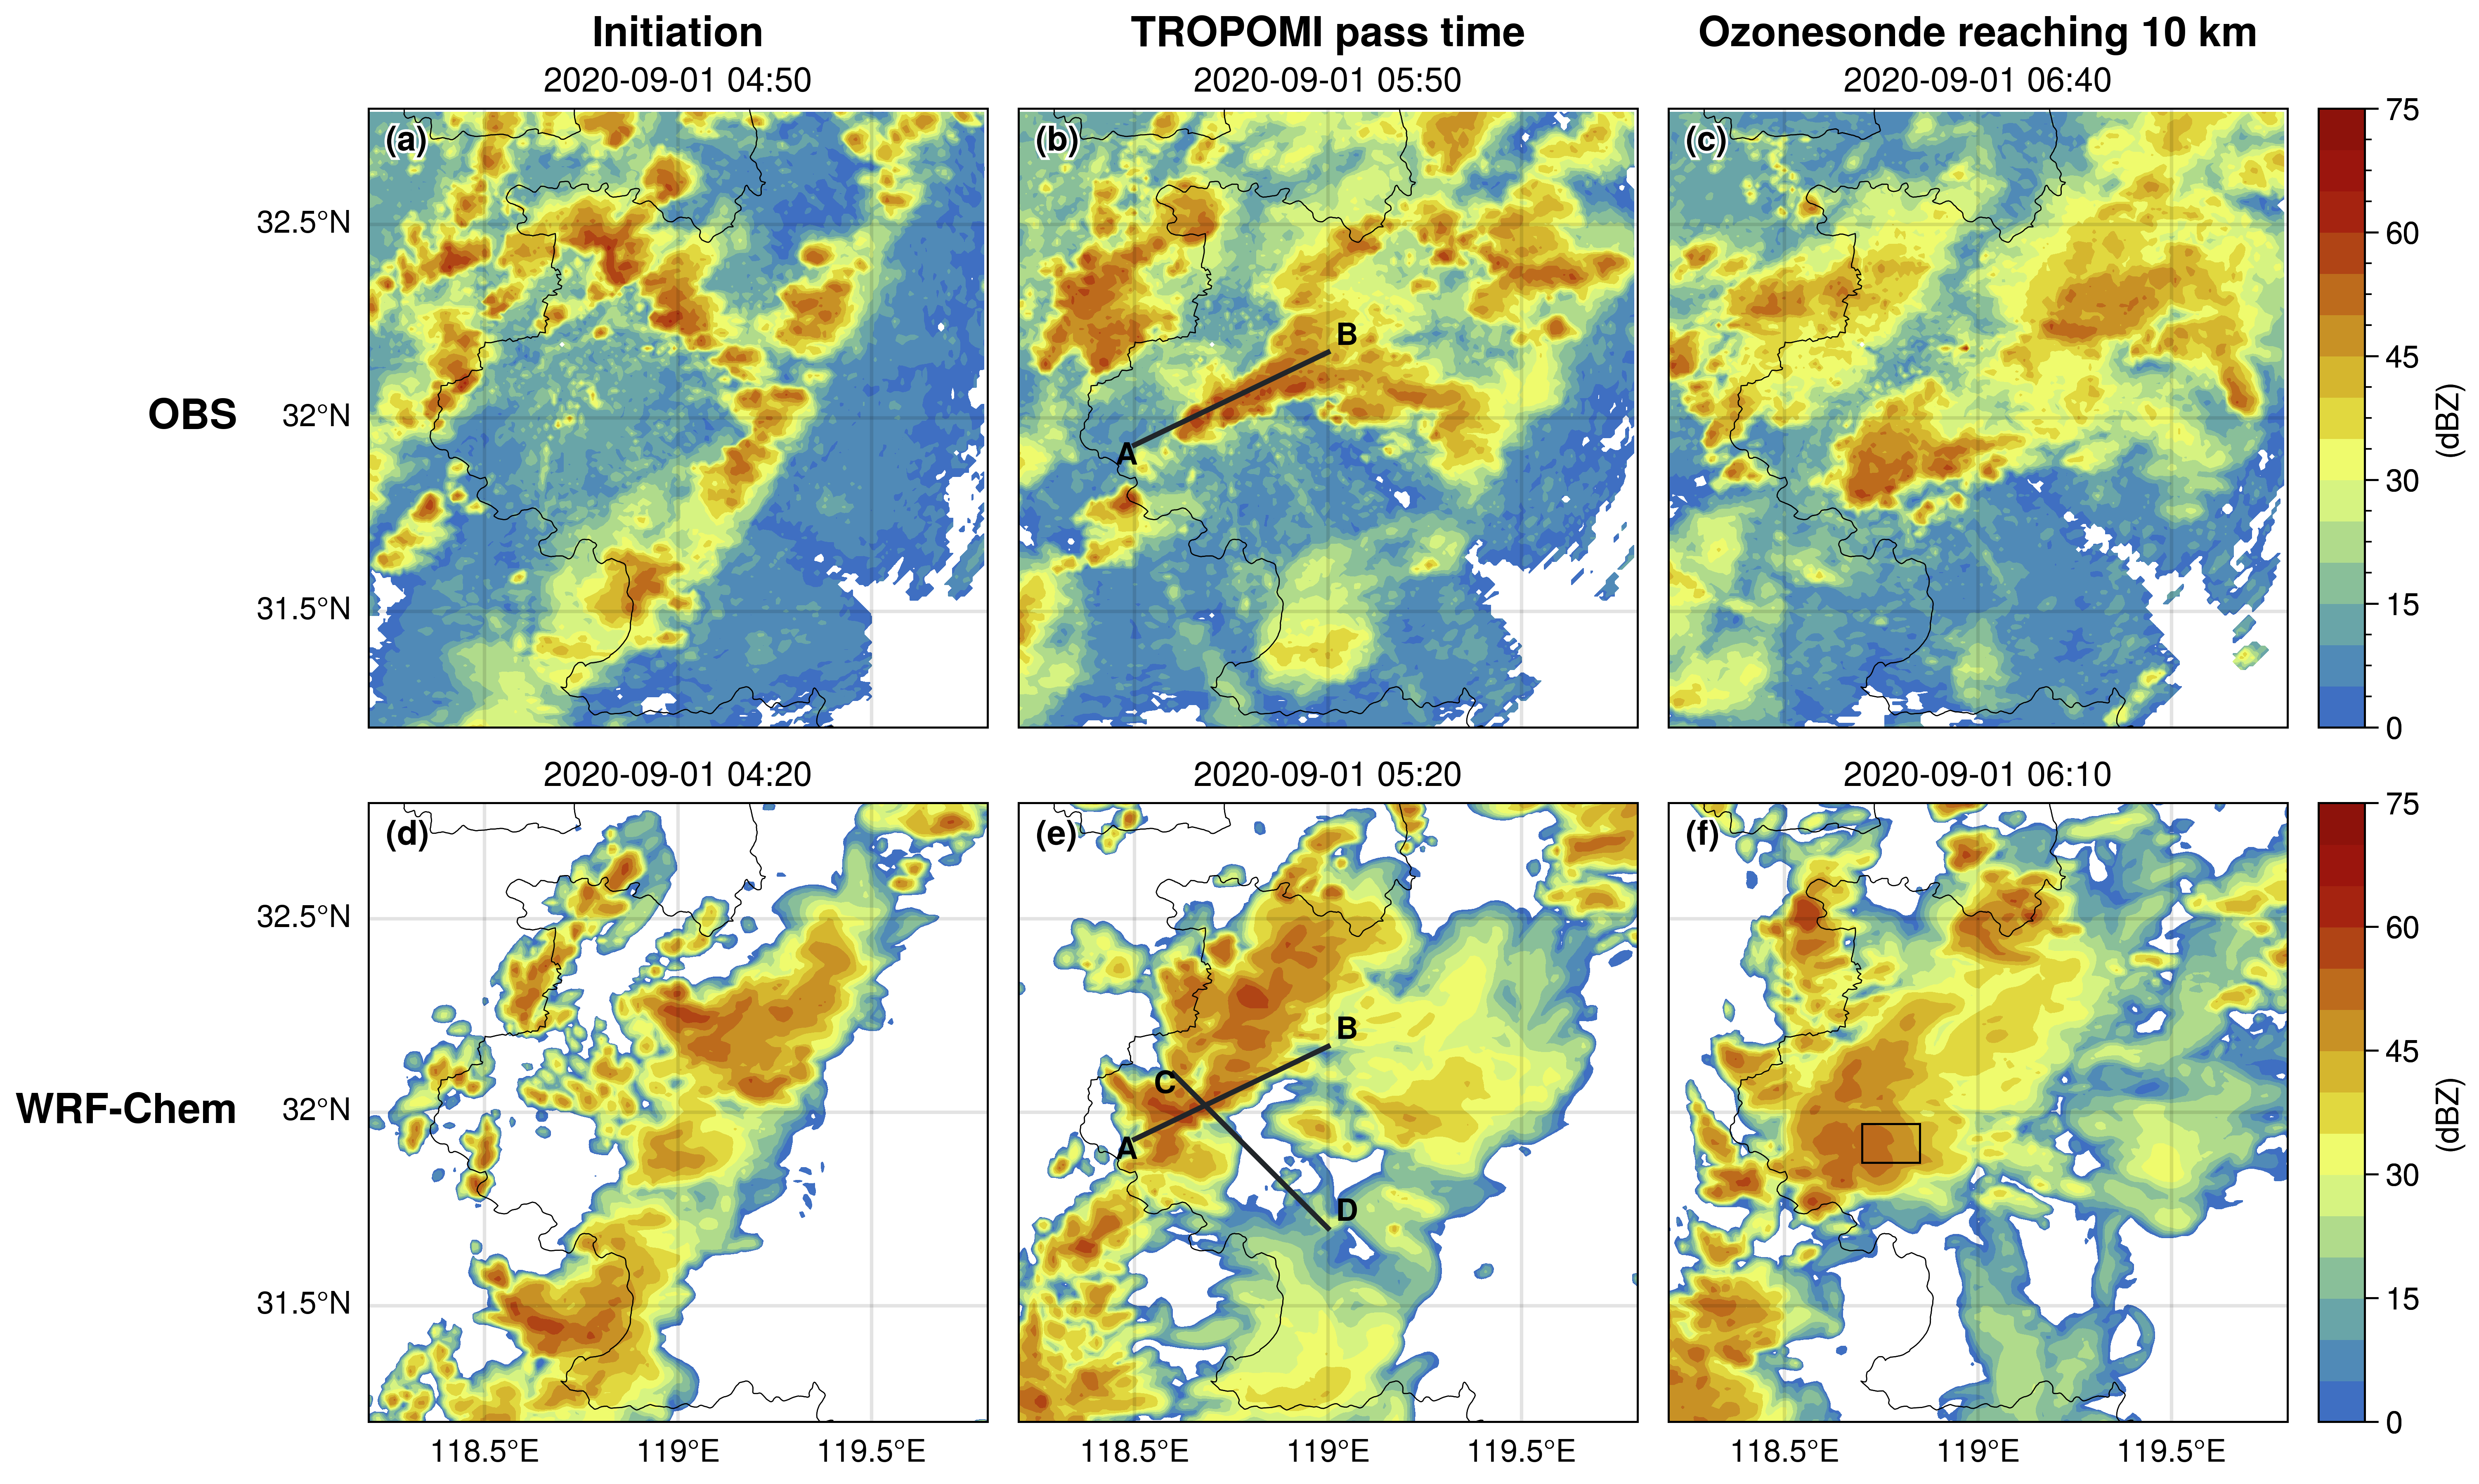
\includegraphics[width=0.9\textwidth]{./figures/comp_crf_2020.png}
\caption{与图\ref{fig:comp_crf_2019} 相同,但针对2020年9月1日的对流个例,模拟时间比雷达观测提前30分钟。\\
Figure \ref{fig:comp_crf_2020}. Same as Fig. \ref{fig:comp_crf_2019} but for the case on 01 September 2020.
The simulation time is 30 minutes ahead of each radar observation.}
\label{fig:comp_crf_2020}
\end{figure}

\begin{figure}[!htbp]
\centering
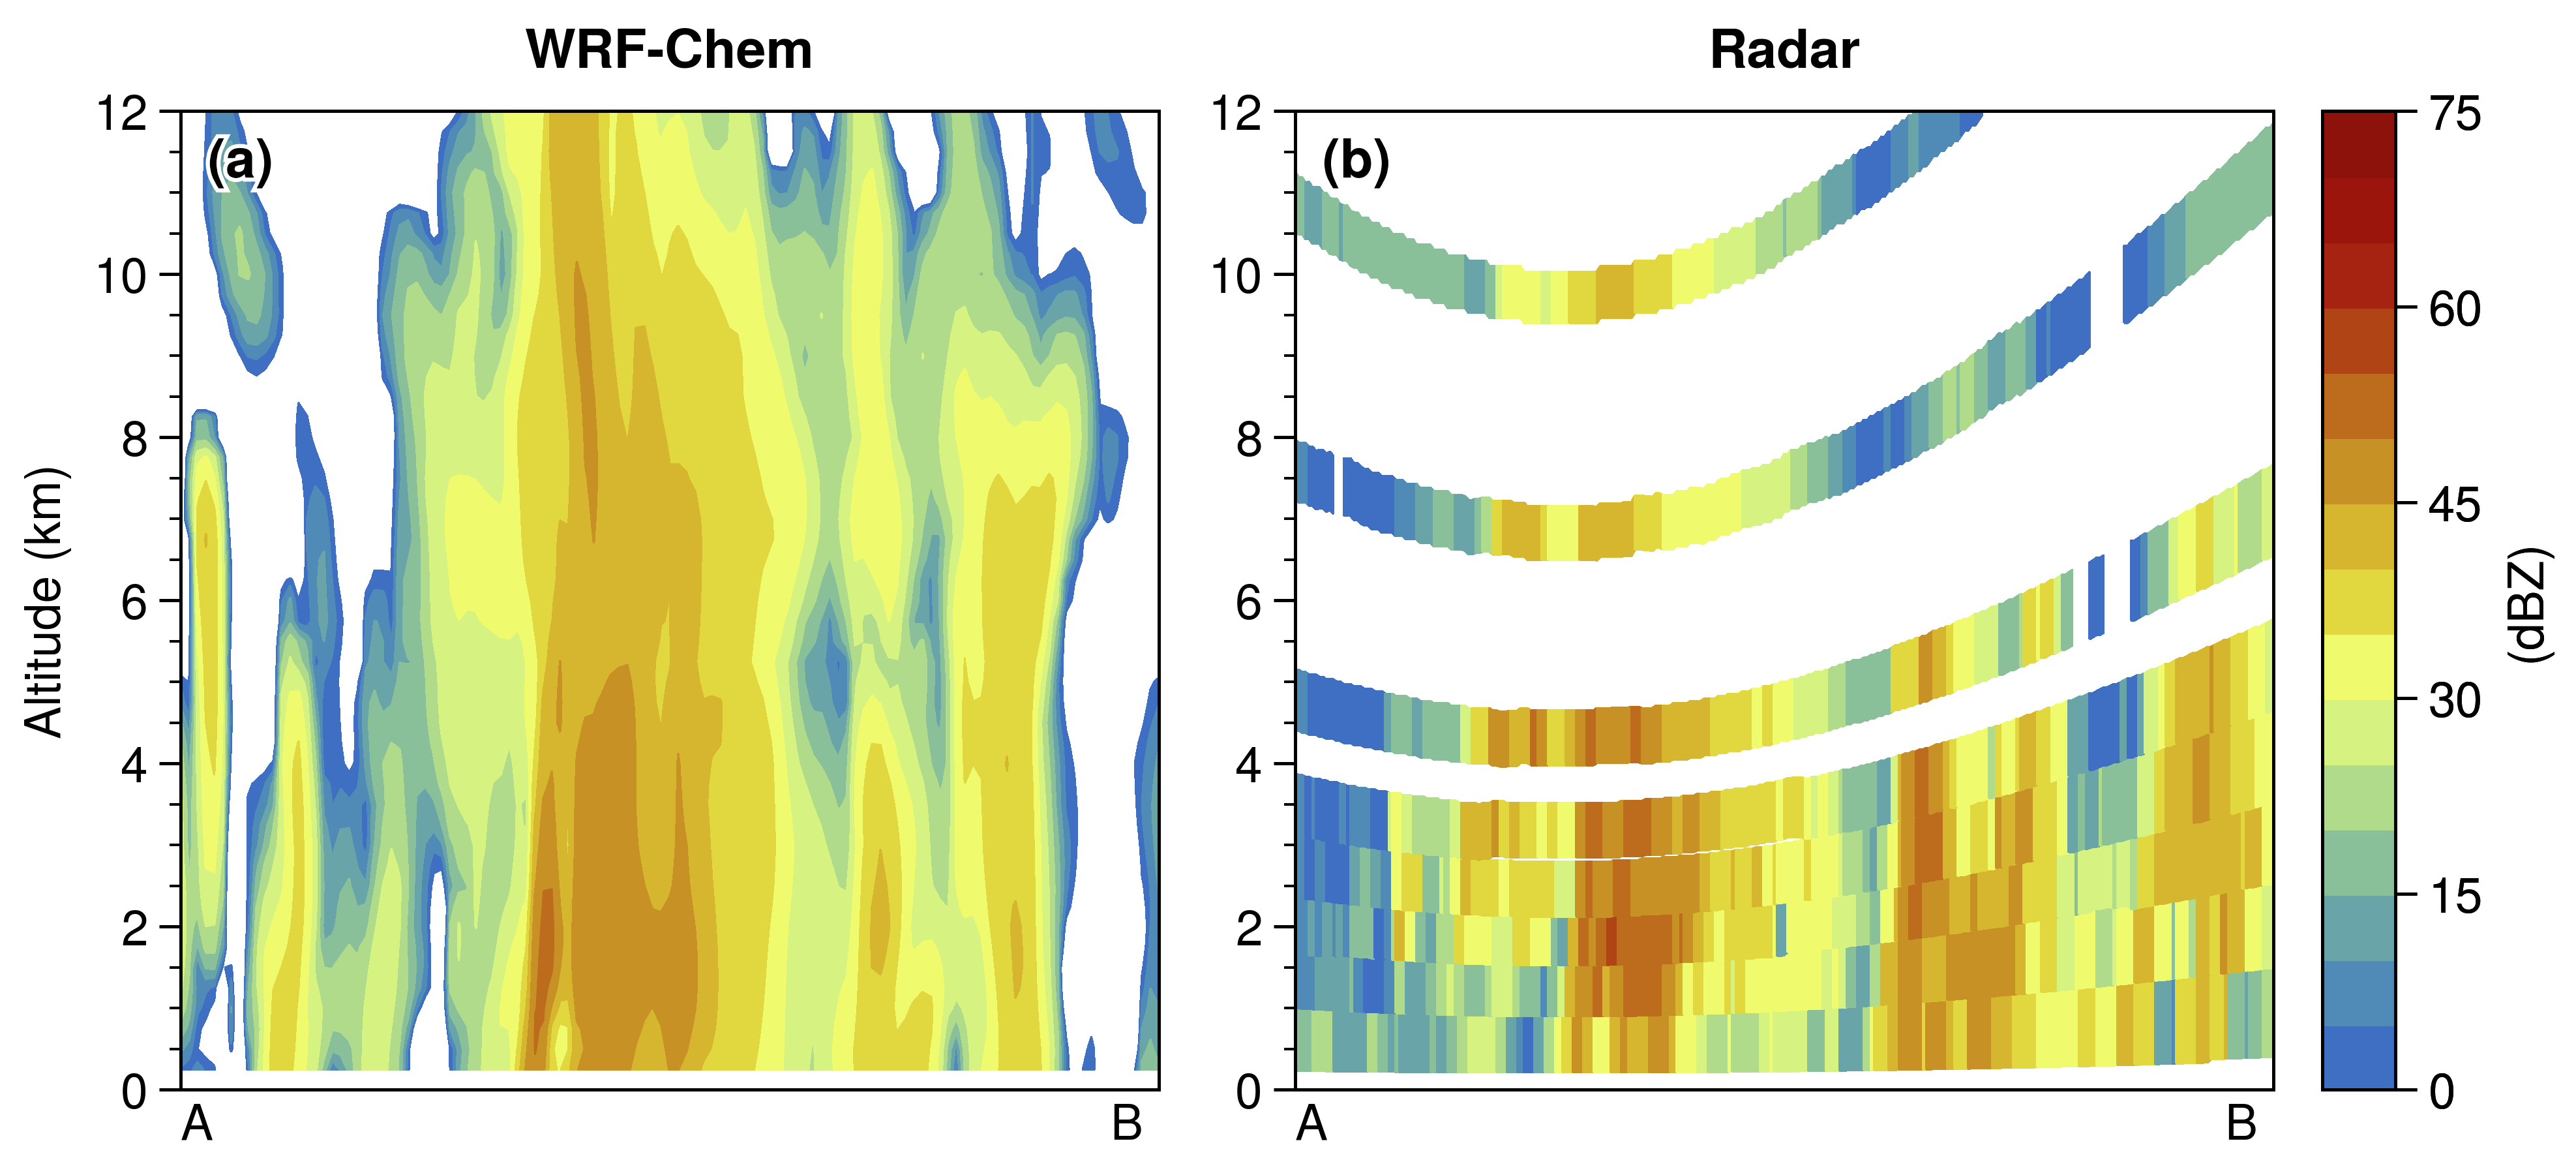
\includegraphics[width=0.8\textwidth]{./figures/comp_dbzcross_2019.png}
\caption{沿着图\ref{fig:comp_crf_2019}中AB线剖得的2019年7月25日(a)WRF-Chem模拟的和(b)雷达观测的雷达反射率。\\
Figure \ref{fig:comp_dbzcross_2019}. Vertical cross sections of (a) WRF-Chem simulated and (b) observed radar reflectivity fields along the transect lines (AB) in Fig. \ref{fig:comp_crf_2019} for 25 July, 2019.}
\label{fig:comp_dbzcross_2019}
\end{figure}

\begin{figure}[!htbp]
\centering
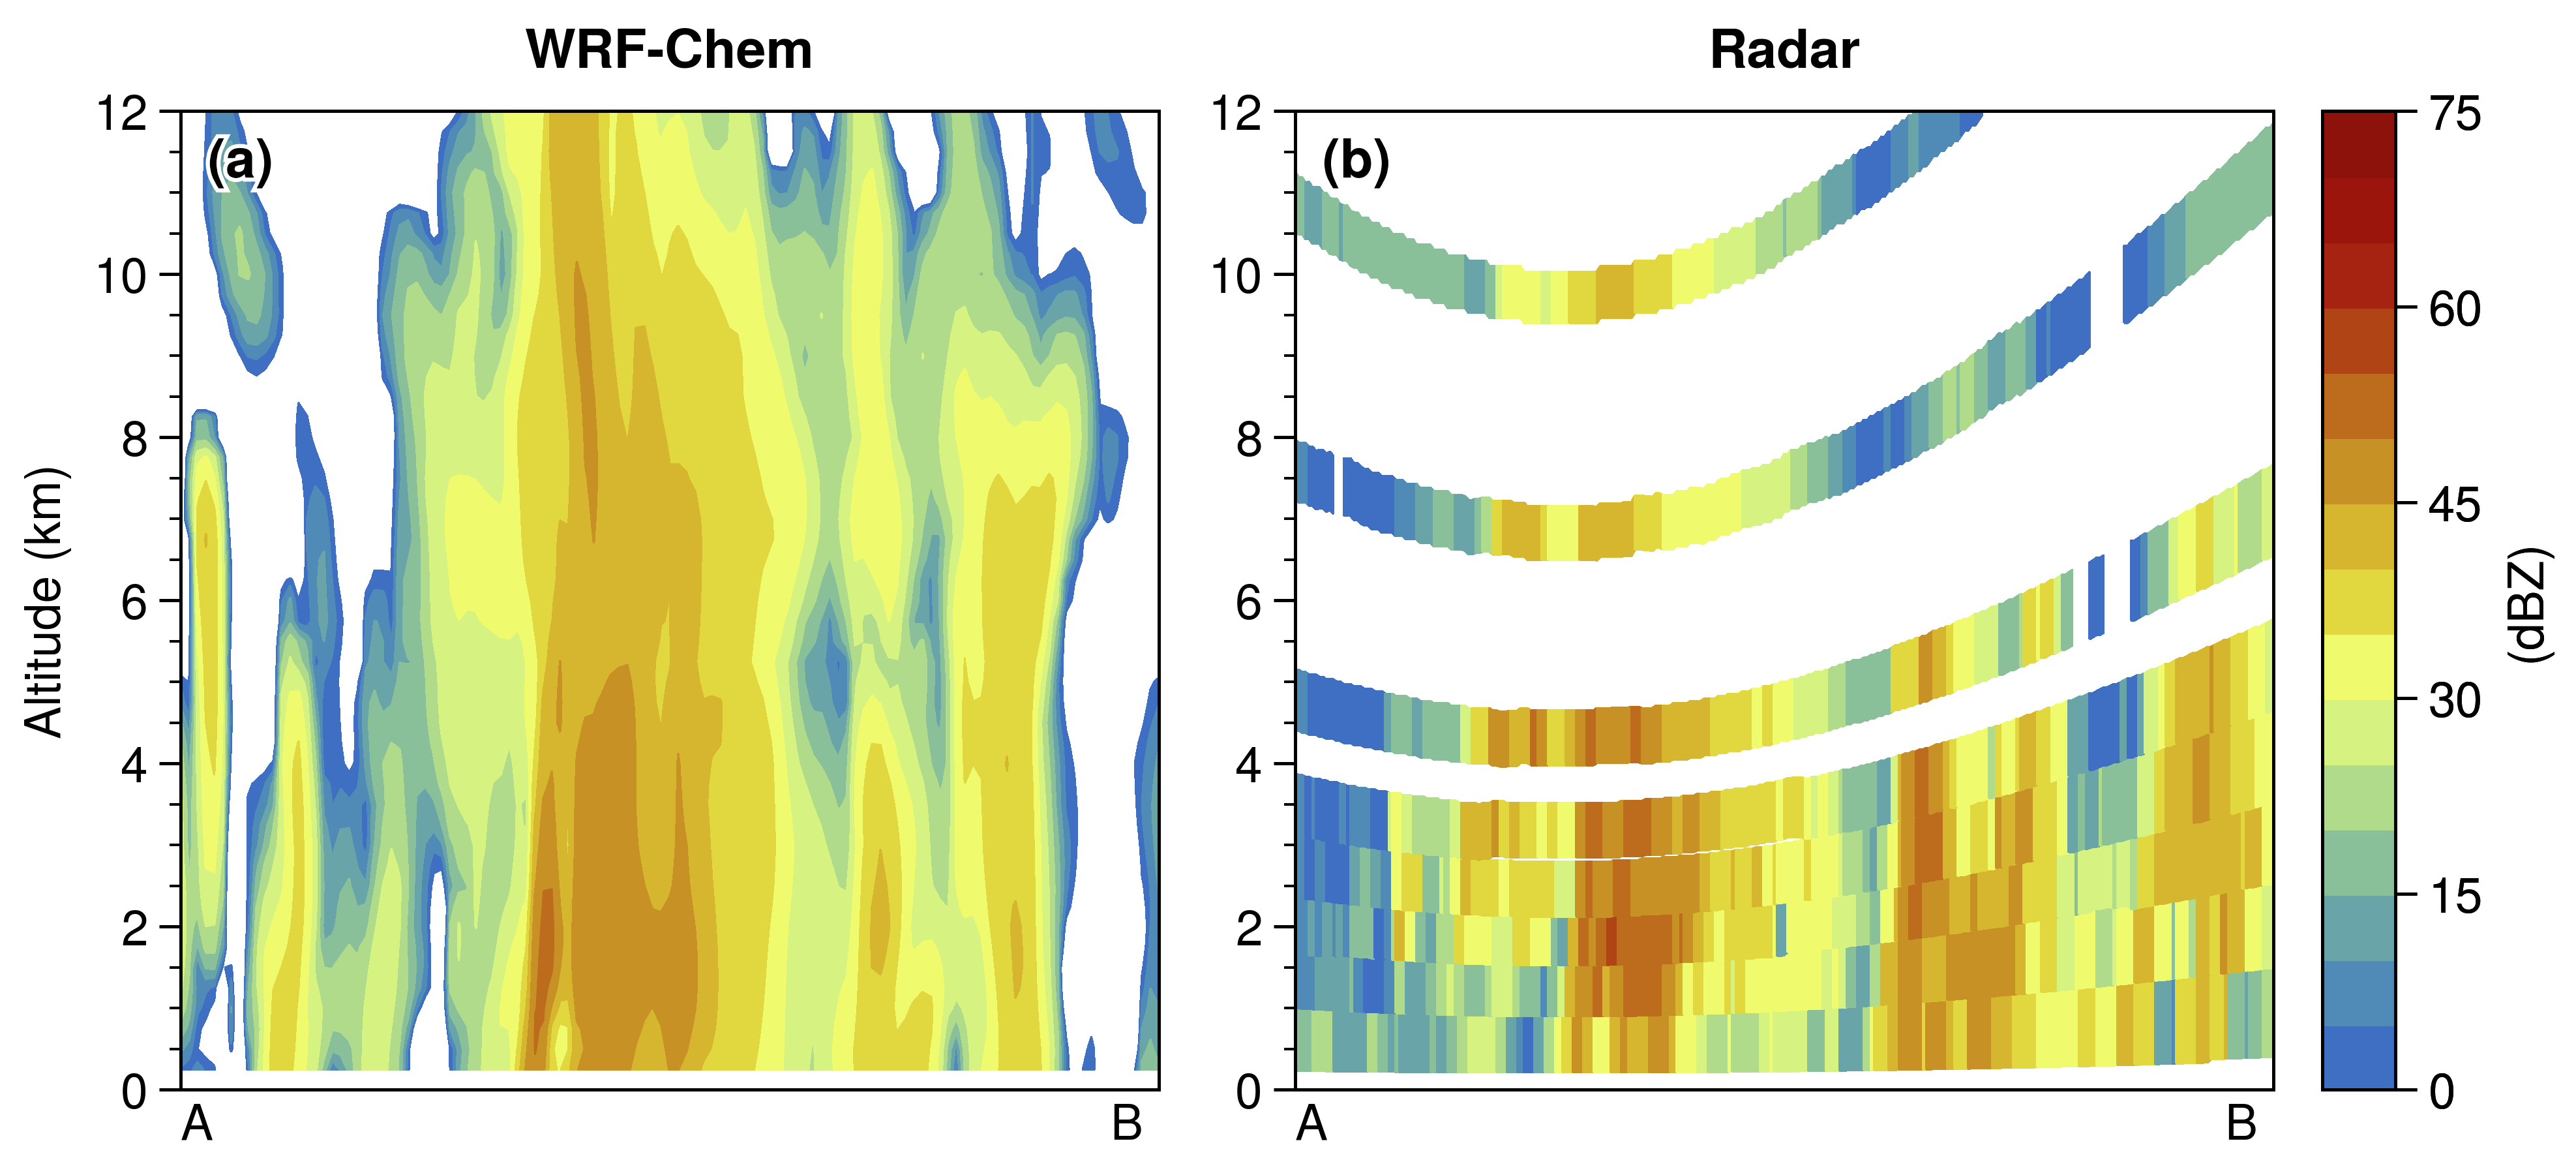
\includegraphics[width=0.8\textwidth]{./figures/comp_dbzcross_2019.png}
\caption{与图\ref{fig:comp_dbzcross_2019}相同,但针对2020年9月1日的对流个例。\\
Figure \ref{fig:comp_dbzcross_2020}. Same as Figure \ref{fig:comp_dbzcross_2019} but for the case on 01 September 2020.}
\label{fig:comp_dbzcross_2020}
\end{figure}



\section{结果与讨论}

\subsection{臭氧的垂直分布} \label{sec:o3_profile}

在不同对流阶段所测的O$_3$和Q$_v$分布如图\ref{fig:ozonesonde_profile}所示。
一般来说,对流导致上对流层O$_3$和Q$_v$浓度增大,且增强的最大值所在区域为10--16 km 之间。
然而,2020年的个例观测显示对流层低层(2--8 km)的O$_3$有较大的增加。
此外,两个个例都存在双谷形状的O$_3$剖面,但高度不同:2019年的热对流个例为2 km和8 km,2020年的飑线为4 km和10 km。
尽管WRF-Chem模型倾向于分别低估2019年和2020年的下对流层和上对流层中的O$_3$浓度,但再现了详细的O$_3$垂直分布结构,故能用以分析对流影响O$_3$的机制。
共有三个来源可以解释上对流层O$_3$的增加:对流输送、化学反应和闪电直接产生的O$_3$。
本研究(\ref{sec:convec_impacts}节)仅详细讨论前两个因素,因为闪电直接产生的O$_3$超出了本研究的范围,并且有限的观测和模式模拟结果显示其产量仍不确定\citep{Morris.2010,Ripoll.2014}。


\begin{figure}[!htbp]
\centering
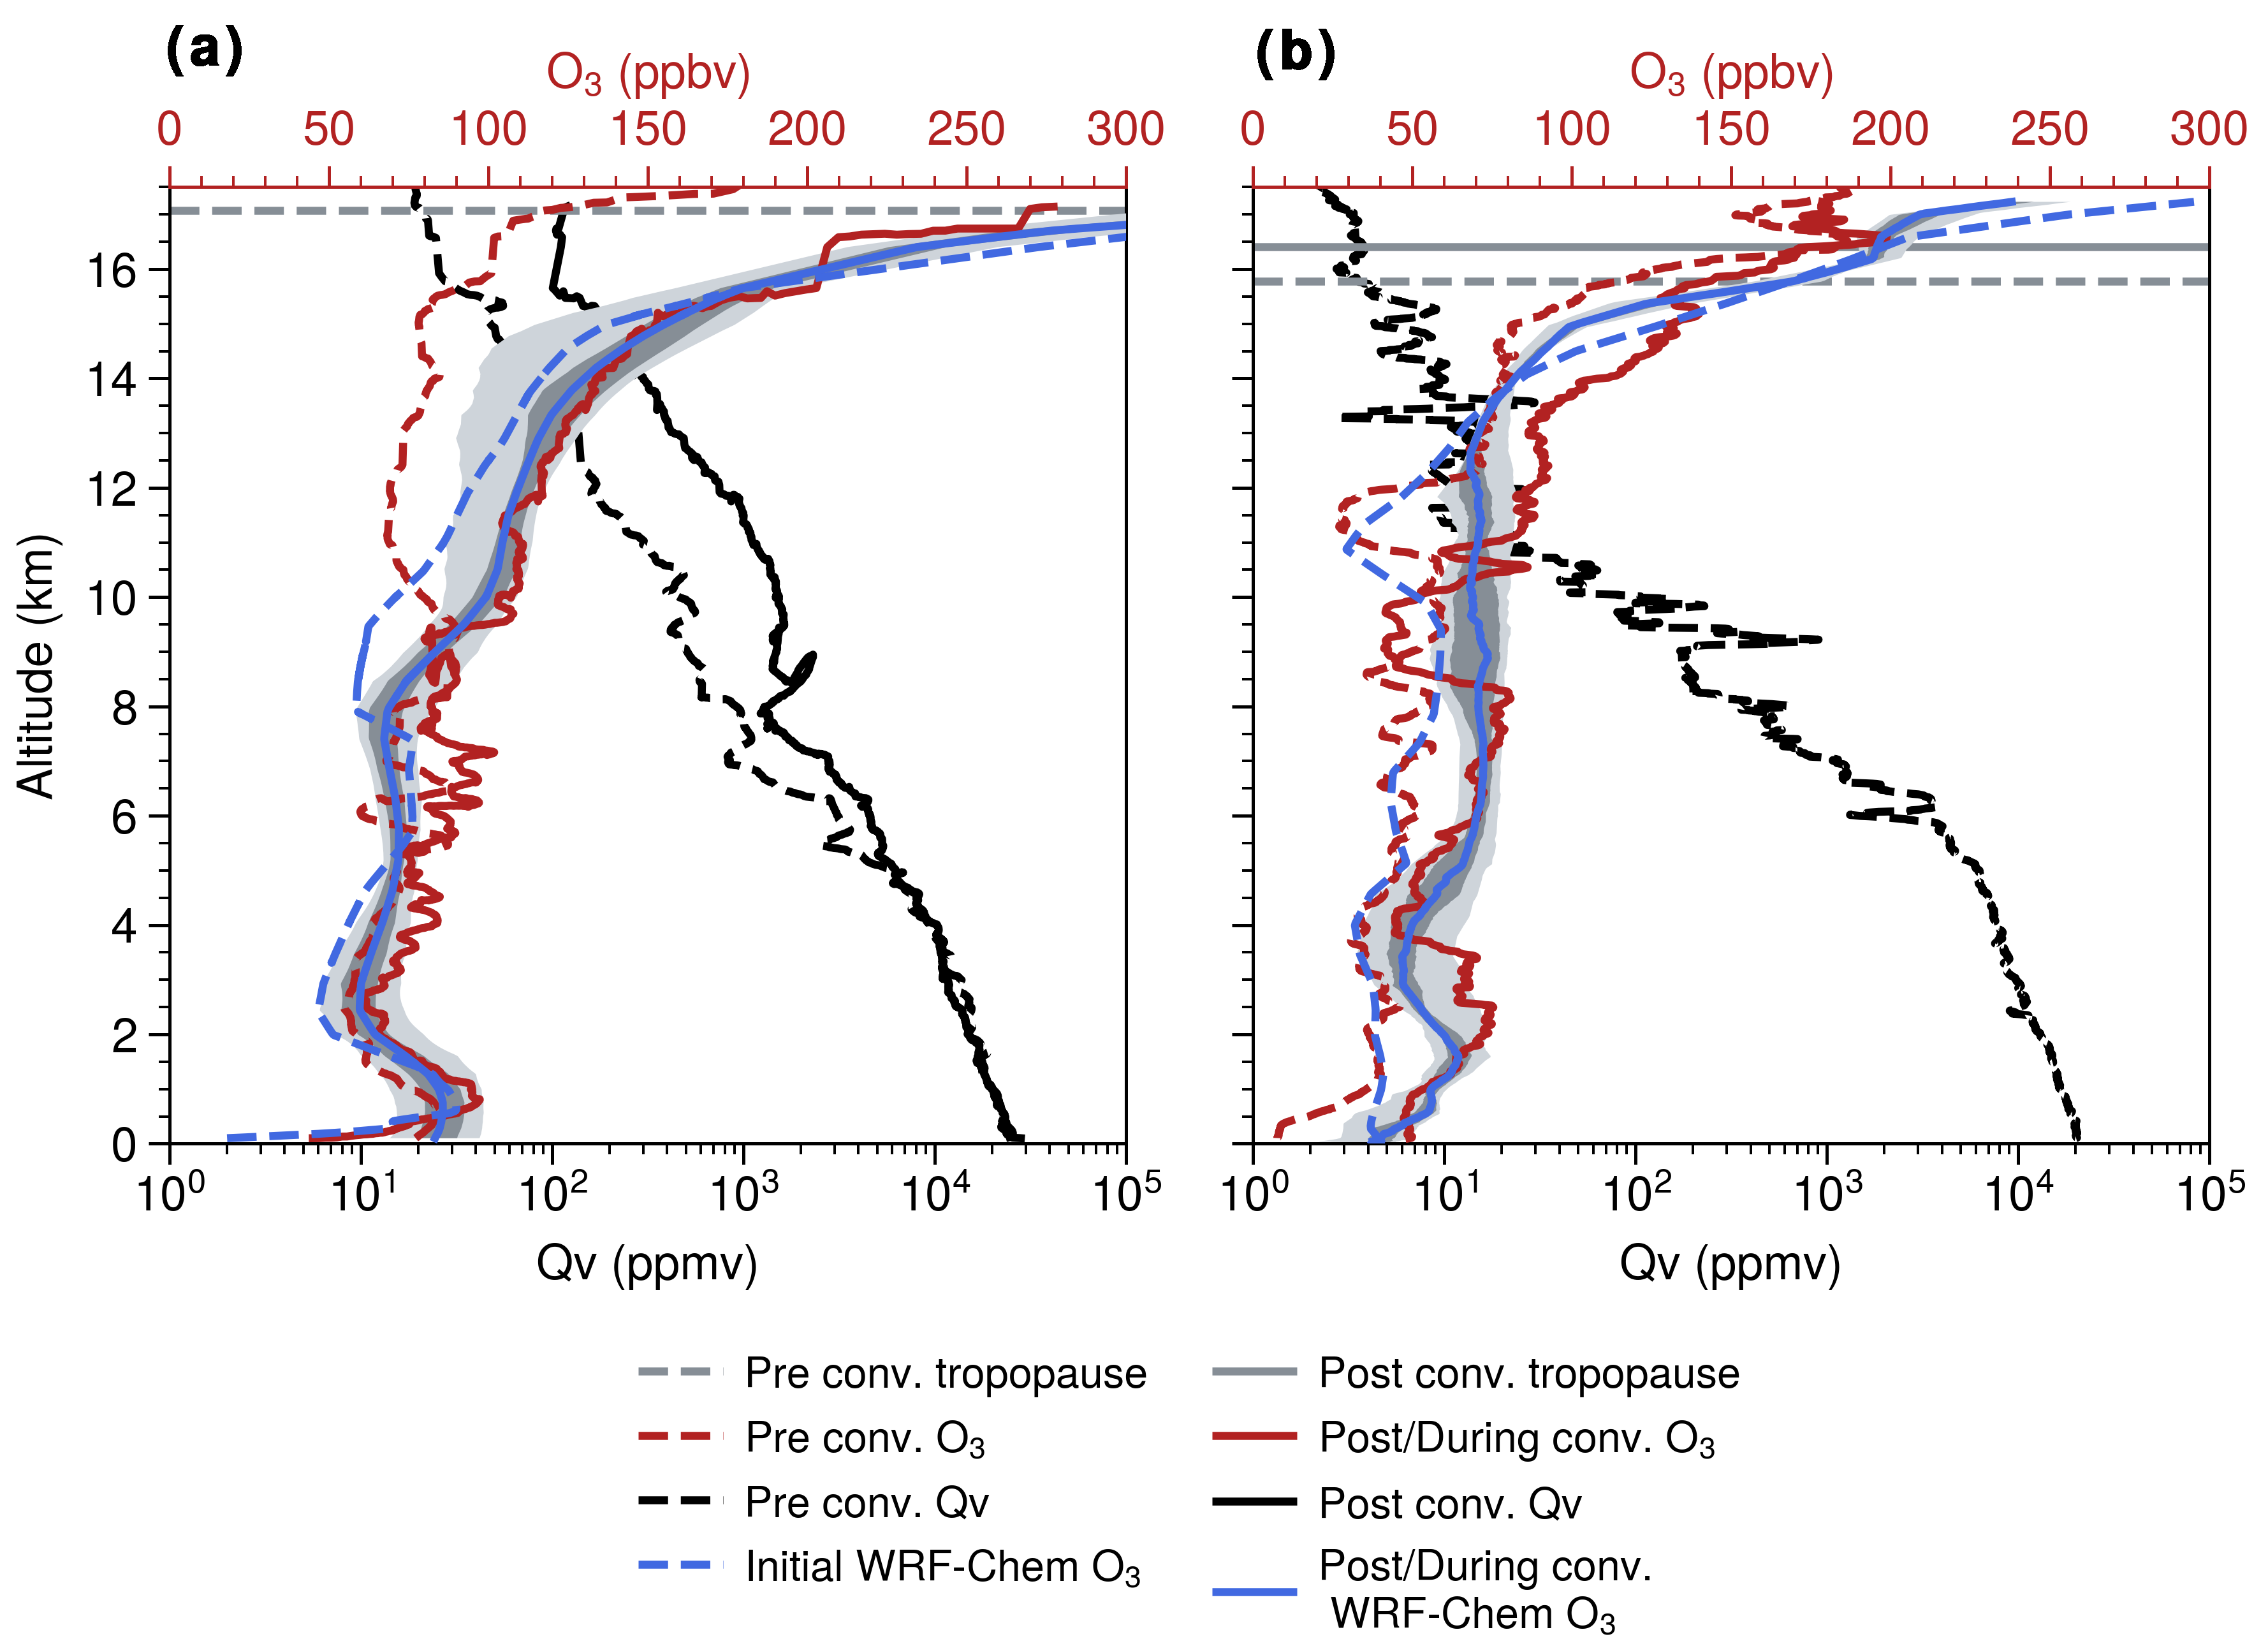
\includegraphics[width=0.8\textwidth]{./figures/ozonesonde_profile.png}
\caption{对流前(虚线)和对流后/对流期间(实线)探空观测到的O$_3$(红色)和Q$_v$(黑色)廓线。
模式初始(虚线)和对流后或对流期间(实线)的O$_3$廓线为蓝色。
深灰色阴影是50\%的置信区间,浅色是90\%的置信区间,灰线是第一对流层顶。\\
Figure \ref{fig:ozonesonde_profile}. Observed O$_3$ (red) and Qv (black) profiles in the pre-convection (dashed) and post-convection/during-convection (solid) periods.
The initial (dashed) and simulated post-convection or during-convection (solid) O$_3$ profiles are in blue.
The dark gray shading is the 50 \% confidence interval while the light one is the 90 \% confidence interval.
The gray lines are the lapse rate tropopauses.
}
\label{fig:ozonesonde_profile}
\end{figure}


除了中国东南部的臭氧探空观测外,我们也利用云切片算法得到了2019年6--8月中低纬度对流云内的O$_3$浓度分布。
如图\ref{fig:uto3_tropomi}所示,TROPOMI云切片方法可得到不同高度O$_3$的平均浓度,
其有效范围比NO$_2$的云切片结果(图\ref{fig:utno2_tropomi})更广,尤其是在中云和高云条件下的中纬度地区(图\ref{fig:uto3_tropomi} b--d)。
这是由于TROPOMI O$_3$二级产品的云分数为光学云识别算法(OCRA)云分数,而NO$_2$二级产品中使用从氧气A波段版本S(FRESCO-S)中快速检索云的方案。
总体上,由于布鲁尔-多普森环流,纬度越高,同一气压层的O$_3$浓度越高。
对于热带地区,非洲中部(20$^{\circ}$ W--50$^{\circ}$ E,0--20$^{\circ}$ N)的O$_3$浓度比同纬度地区的O$_3$浓度高,尤其是在中云和高云条件下可高出40\%--48\%,该现象与\citet{Cooper.2013}研究中215 hPa高度MLS的O$_3$观测结果相符。
他们的研究指出,低O$_3$事件经常发生在热带西太平洋,很少发生在热带其他地区,
而热带海洋区域在低O$_3$事件和高云的频率之间存在一致的空间特征,表明这些事件来自于对流。
虽然非洲中部也是强对流频发地区,但陆地边界层O$_3$浓度往往高于海洋,因此深对流产生较少的低O$_3$事件。
此外,高云处的O$_3$浓度(图\ref{fig:uto3_tropomi}(a--b))高于中云(图\ref{fig:uto3_tropomi}(c--d)),
其中180 hPa--330 hPa间的O$_3$为330 hPa--450 hPa间的$\approx$1.5倍,为450--570 hPa间的$\approx$2倍。

为了进一步利用MERRA2-GMI的模式结果分析动力输送和化学反应在其中的作用,我们首先将各个高度的MERRA2-GMI模式结果与TROPOMI观测数据相比较。
图\ref{fig:uto3_merra2}为2019年6--8月与TROPOMI对应的MERRA2-GMI O$_3$模拟结果,
图\ref{fig:uto3_delta}为TROPOMI与MERRA2-GMI在各层的结果之差($\Delta$ O$_3$)。
总体上,非洲中部的$\Delta$ O$_3$在中云和高云条件下为负(可小于-20 pptv,图\ref{fig:uto3_delta} a--d),中纬度地区的$\Delta$ O$_3$在高云条件下为正(可大于 40 pptv,图\ref{fig:uto3_tropomi} b),
该两处之外的$\Delta$ O$_3$绝对值均小于10。
此外,通过对比$\Delta$ NO$_2$(图\ref{fig:utno2_tropomi})和$\Delta$ O$_3$(图\ref{fig:uto3_delta}),
我们发现由于清洁的上对流层属于NO$_x$控制区\citep{Brown.2022},因此MERRA2-GMI的NO$_2$较TROPOMI高估,导致MERRA2-GMI的O$_3$亦高估。
只有在$\Delta$ NO$_2$ $>$ 60 pptv的条件下,$\Delta$ O$_3$ $>$ 10 pptv(图\ref{fig:uto3_delta} a--b),
在$\Delta$ NO$_2$ $<$ -10 pptv的条件下,$\Delta$ O$_3$ $<$ -40 pptv,该现象与NO$_x$控制区内EKMA曲线在低NO$_x$值区更密集的结论相符。
低云条件下的云切片O$_3$的低估,也反映了几何AMF(AMF$_{geo}$)在低云和污染条件下的高估\citep{BelmonteRivas.2015}。

\begin{figure}[!htbp]
    \centering
    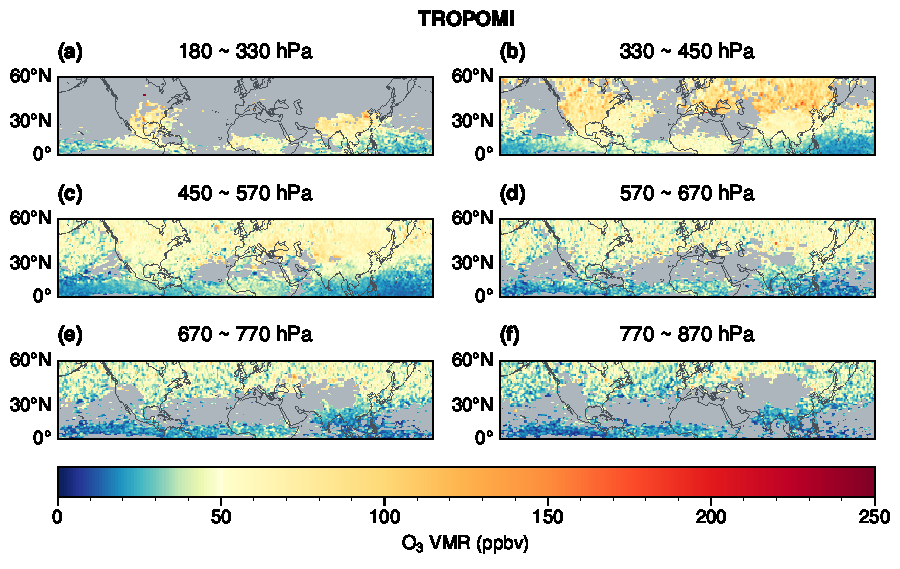
\includegraphics[width=15cm]{./figures/uto3_tropomi.pdf}
    \caption{
    TROPOMI云切片算法所得的2019年6--8月北半球中低纬度O$_3$浓度分布图。 \\
    Figure \ref{fig:uto3_tropomi}. The O$_3$ vertical mixing ratios derived from the cloud-slicing results of TROPOMI O$_3$ observations at the northern middle and low latitudes for June--August in 2019.
    }
    \label{fig:uto3_tropomi}
\end{figure}


\begin{figure}[!htbp]
    \centering
    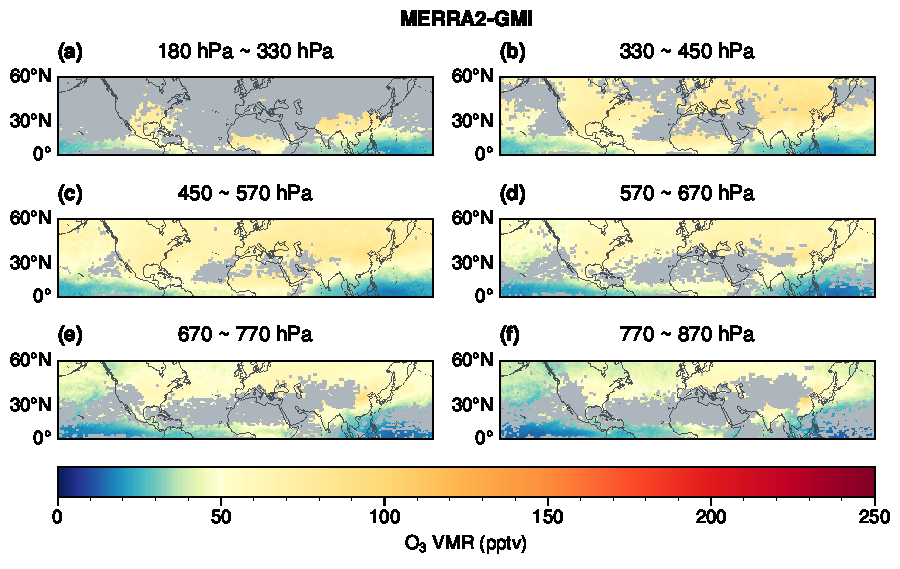
\includegraphics[width=15cm]{./figures/uto3_merra2-gmi.pdf}
    \caption{
    同图\ref{fig:uto3_tropomi}但数据为MERRA2-GMI。 \\
    Figure \ref{fig:uto3_merra2}. Same as Fig. \ref{fig:uto3_tropomi} but for MERRA2-GMI.
    }
    \label{fig:uto3_merra2}
\end{figure}


\begin{figure}[!htbp]
    \centering
    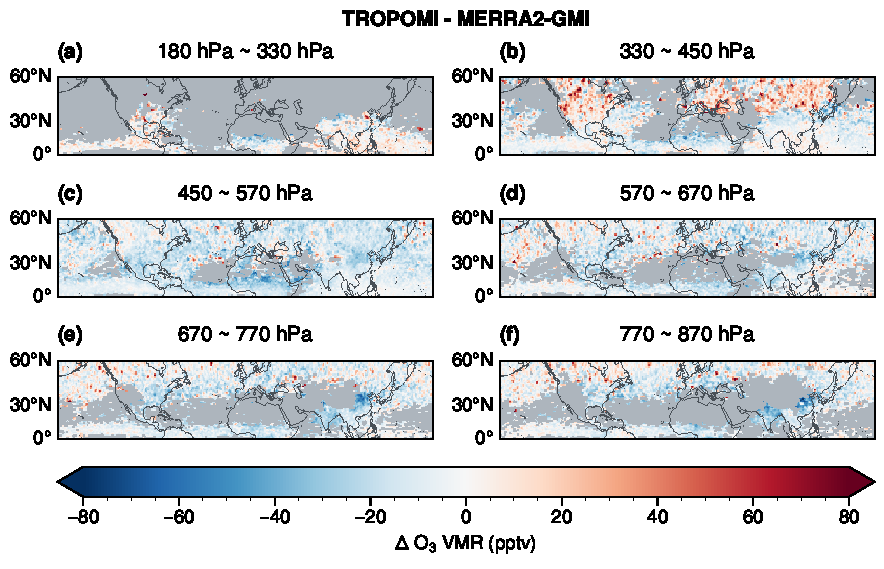
\includegraphics[width=15cm]{./figures/uto3_delta.pdf}
    \caption{
    图\ref{fig:uto3_tropomi}与图\ref{fig:uto3_merra2}之差。 \\
    Figure \ref{fig:uto3_delta}. Differences between Fig. \ref{fig:uto3_tropomi} and Fig. \ref{fig:uto3_merra2}.
    }
    \label{fig:uto3_delta}
\end{figure}


鉴于高云条件下的云切片结果在中纬度地区有效数较少(图\ref{fig:uto3_tropomi}a),
我们将MLS于261 hPa高度观测的O$_3$浓度与MERRA2-GMI的O$_3$模拟结果,在晴空和有云条件下分别进行对比。
如图\ref{fig:mls_o3_261hpa}所示,在低纬度地区两者均显示有云条件下海洋上O$_3$浓度较晴空降低5\%--60\%,而非洲中部和印度北部的O$_3$浓度较晴空增大1\%--46\%。
晴空条件下两者在中纬度地区的O$_3$浓度一致,但有云时两者的变化相反,具体而言,MLS观测显示有云条件下261 hPa高度的O$_3$浓度比晴空时的浓度高,而MERRA2-GMI模拟显示O$_3$浓度比晴空时的浓度低。
在40--60$^{\circ}$ N区域内有高云的条件下,MERRA2-GMI模拟的O$_3$平均浓度为108 ppbv,与TROPOMI云切片得到的O$_3$平均浓度(86 ppbv)相接近,而MLS的平均观测结果(230 ppbv)为MERRA2-GMI和TROPOMI的2--3倍。
MLS的O$_3$廓线在上对流层的分辨率为3--6 km,而261 hPa所在高度接近于中纬度地区的对流层顶高度,故过度的外推可能导致MLS测得的O$_3$浓度过高\citep{Schoeberl.2007}。


\begin{figure}[!htbp]
    \centering
    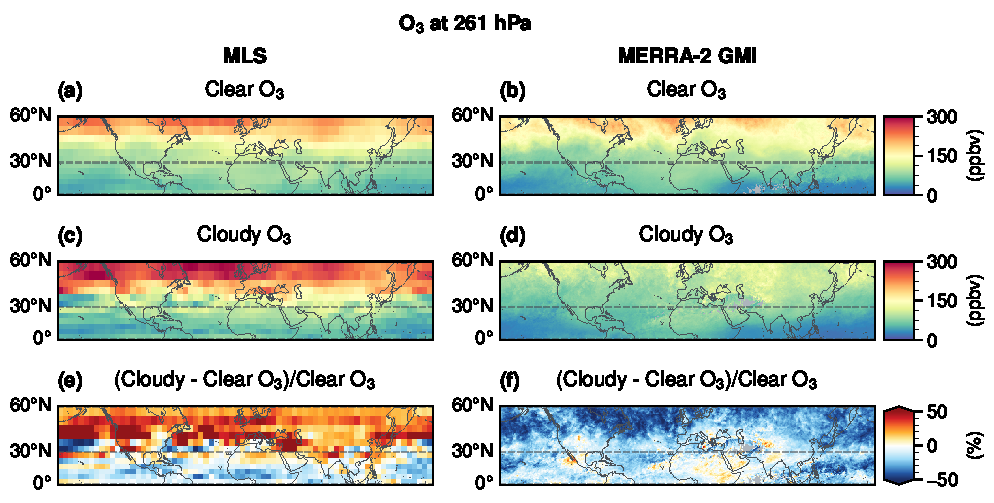
\includegraphics[width=15cm]{./figures/mls_o3_261hpa.pdf}
    \caption{
    2019年6--8月北半球中低纬度晴空(a--b)和有云(c--d)条件下261 hPa高度O$_3$的平均浓度,以及相对百分比变化(e--f)。
    第一列为MLS观测数据,第二列为MERRA2-GMI模拟结果。 \\
    Figure \ref{fig:mls_o3_261hpa}. The mean O$_3$ concentrations at 261 hPa with clear (a--b) and cloudy (c--d) conditions at the northern middle and low latitudes for June--August in 2019. The percentage differences are shown in panel (e) and (f).
    The first column is the MLS observations while the second column is the MERRA2-GMI simulations.
    }
    \label{fig:mls_o3_261hpa}
\end{figure}


除了各层O$_3$浓度的地理分布之外,我们选取了区域内云切片有效层数为6层的格点(中国南部、印度中部、美国东南部、以及太平洋,图\ref{fig:no2_ltngcount}a),
进行MERRA2-GMI和TROPOMI的廓线对比分析。
如图\ref{fig:uto3_profile}所示,O$_3$浓度在中云和高云的条件下随着高度升高而降低,
但是由于几何AMF的限制,低云条件下的O$_3$浓度在中国南部、印度中部、和美国东南部没有显示出O$_3$的高值,故接下来只比较MERRA2-GMI和TROPOMI在对流层中上层的O$_3$浓度。
对于中国南部和印度中部,MERRA2-GMI的模拟值高于TROPOMI的观测值,两者之差从570--670 hPa的20 pptv逐渐下降至180--330 hPa的2 pptv。
对于美国东南部,TROPOMI的观测值在330--450 hPa间有一峰值,与图\ref{fig:utno2_profile}c中LNO$_2$峰值相对应,
而MERRA2-GMI的模拟结果在该高度不存在O$_3$峰值,即MERRA2-GMI上对流层LNO$_2$的差异导致O$_3$的低估。
对于清洁的太平洋地区,两者随高度而降低的趋势一致,且误差小于5 pptv。
总之,TROPOMI的观测结果和MERRA2-GMI的模拟结果在对流层中上层存在显著的一致性,
局部的差异表明云切片方法可以用来检验模式中LNO$_x$的产量和影响。



\begin{figure}[!htbp]
    \centering
    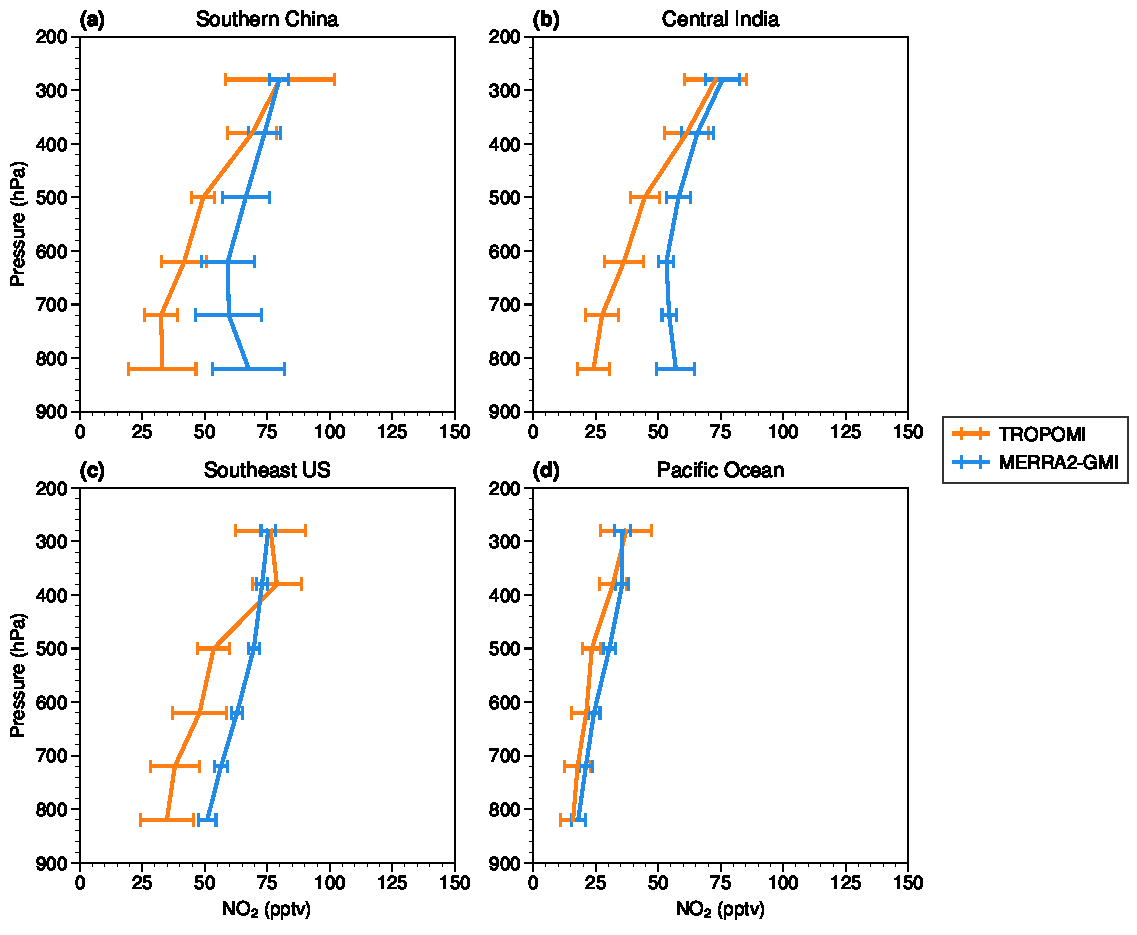
\includegraphics[width=12cm]{./figures/uto3_profile.pdf}
    \caption{
    MERRA2-GMI(蓝色)和TROPOMI云切片算法(橙色)所得到的区域平均O$_3$廓线
    (a)中国南部、(b)印度中部、(c)美国东南部、(d)太平洋(区域示意图见图\ref{fig:no2_ltngcount}a)。
    其中廓线的误差棒为平均值$\pm$标准差。\\
    Figure \ref{fig:uto3_profile}. Regional average NO$_2$ profiles obtained by MERRA2-GMI (blue) and TROPOMI cloud slice algorithm (orange)
    (a) southern China, (b) central India, (c) southeastern United States, and (d) Pacific Ocean
    (Definitions of region are shown in Fig. \ref{fig:no2_ltngcount}a).
    where the error bars are the mean values $\pm$ standard deviations.
    }
    \label{fig:uto3_profile}
\end{figure}


\subsection{动力输送和化学反应的贡献} \label{sec:convec_impacts}

为了探究中国东南部对流后上对流层O$_3$浓度增大的原因,我们将对流分为三个阶段(初生、发展和消散)来分析臭氧探空仪所经区域中O$_3$平均浓度的垂直廓线变化(图\ref{fig:tendency_o3}a 和 d)。
其中,2020年个例的上对流层O$_3$在整个周期内一直在增加,而2019年的个例由于发展阶段低浓度O$_3$空气的抬升,O$_3$浓度降低,接着又开始增大,这种现象可以用发展阶段的O$_3$垂直剖面来解释(图\ref{fig:tendency_o3}b和e)。
在2019年的个例中,低O$_3$浓度的空气块通过上升气流达到16 km,然后对流后方的高O$_3$浓度空气被夹卷进该区域。
而2020年个例中观测到增加的O$_3$,主要来自垂直传输的背景O$_3$浓度。

为了确定两种影响之间的差异,我们分析了对流期间10--14 km的平均累计物理变化速率 (IPR,图\ref{fig:tendency_o3}c和f)。
一般来说,水平平流 (advh) 和垂直平流 (advz) 的相反趋势支配着2019年上对流层O$_3$产率的净下降。
其中强上升气流使得低O$_3$浓度的空气块得以抬升,故垂直平流(advz)的贡献在10--11.5 km之间为负,而在11.5到13.8km 之间为正,即存在向下输送的高浓度O$_3$。
此外,由于2020年对流个例发生后的Q$_v$较高(图\ref{fig:ozonesonde_profile}a)且对流层顶高于云区(图\ref{fig:tendency_o3}b),
所以其上升气流不足以像中尺度对流系统一样将平流层高浓度的O$_3$挟至对流层\citep{Phoenix.2020}。
虽然动力输送在O$_3$的变化中起着重要作用,但不能忽视正的化学贡献,尤其是2020年对流期间上对流层O$_3$的净增加。
具体来说,在两次个例中化学反应对O$_3$起到了正贡献,其影响程度是动力输送的5--10倍,这表明化学贡献在对流的整个生命期中占主导地位。


\begin{figure}[!htbp]
\centering
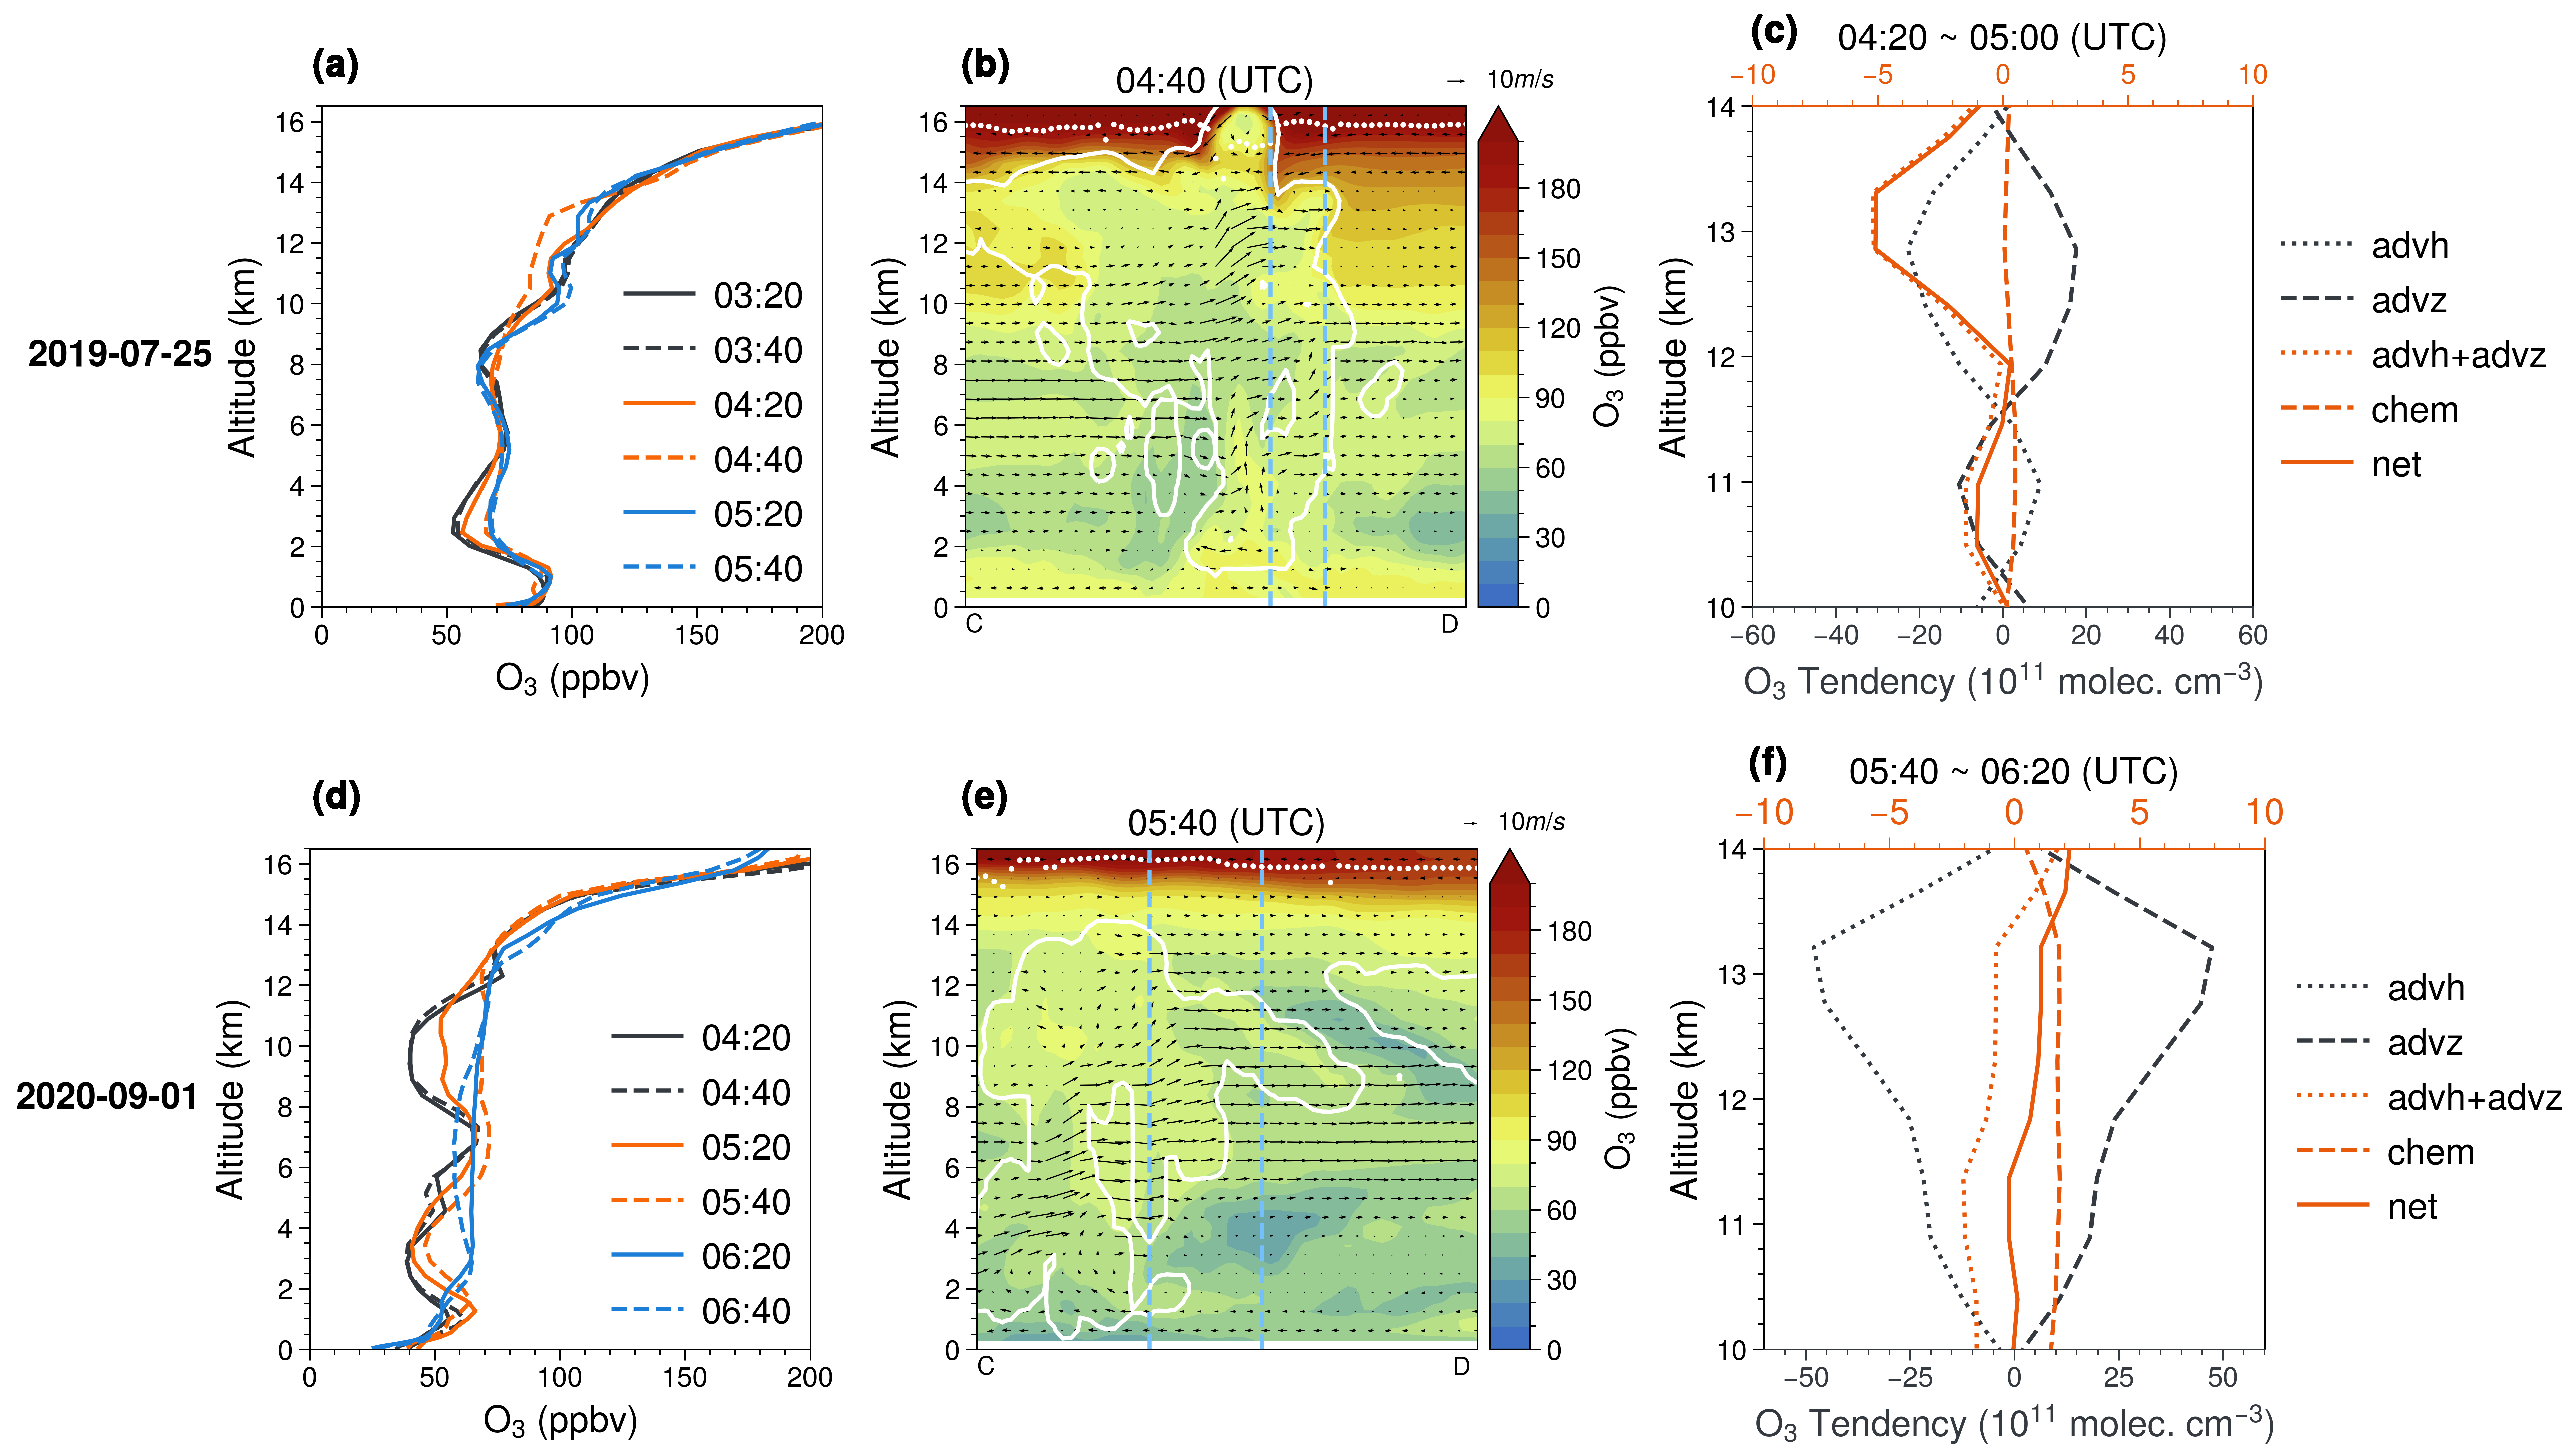
\includegraphics[width=\textwidth]{./figures/tendency_o3.png}
\caption{
(a, d) 臭氧探空仪经过区域的O$_3$平均浓度剖面,包括三个阶段:初生(黑色)、发展(橙色)和消散(蓝色)。
(b,e)对流旺盛期内沿穿过对流核心(图 \ref{fig:comp_crf_2019}e 和图 \ref{fig:comp_crf_2020}f)的O$_3$剖面。
蓝色虚线代表臭氧探空仪经过区域的边界,第一对流层顶显示为白点。
白线为云边界(云液态水混合比[q$_{cloud}$]和冰混合比[q$_{ice}$]之和 $\geq$ 0.01 g/kg)。
(c, f) 对流旺盛期的水平平流 (advh)、垂直平流 (advz) 和化学贡献 (chem)引起的O$_3$净生产率和趋势的垂直分布。
\\
Figure \ref{fig:tendency_o3}. (a, d) The mean O$_3$ profiles in the regions passed by the ozonesondes
at three stages: initiation (black), development (orange), and dissipation (blue).
(b, e) Vertical O$_3$ distribution within the convective periods along the line crossing the convective core (Fig. \ref{fig:comp_crf_2019}e and Fig. \ref{fig:comp_crf_2020}f).
The blue dashed lines stand for the boundaries of regions passed by the ozonesondes, and the lapse rate tropopause is shown as the white dots.
The cloud boundaries (the sum of cloud liquid water mixing ratio [q$_{cloud}$] and ice mixing ratio [q$_{ice}$] $\geq$ 0.01 g/kg) are shown in white lines.
(c, f) The vertical distributions of the O$_3$ net production rate and tendency due to horizontal advection (advh), vertical (advz) advection, and chemistry (chem) during the convective periods.
}
\label{fig:tendency_o3}
\end{figure}


由以上的中国东南部O$_3$变化的分析可知化学贡献的重要性,
因此我们进一步利用MERRA2-GMI的3小时平均模式结果,分析了动力(大尺度输送)、物理(湍流和对流)和化学对中低纬度臭氧的贡献。
如图\ref{fig:uto3_tendency}所示,中低纬度的臭氧趋势由动力项主导,且噪点较多,
物理的贡献主要为负,代表低O$_3$浓度的空气向上对流层输送。
然而在污染地区(如美国东南部、非洲中部、印度北部、以及中国东南部)化学贡献的正贡献占主导,表明净臭氧产生。
由于对流和闪电产生的较高浓度的LNO$_2$,这些区域的正化学贡献在阴天比晴天强50\%--160\%(图\ref{fig:uto3_chem_tendency})。
该结果与中国东南部O$_3$在整个对流生命期的变化及来源相符,突出了LNO$_2$对于夏季上对流层O$_3$浓度的长期影响。

\begin{figure}[!htbp]
    \centering
    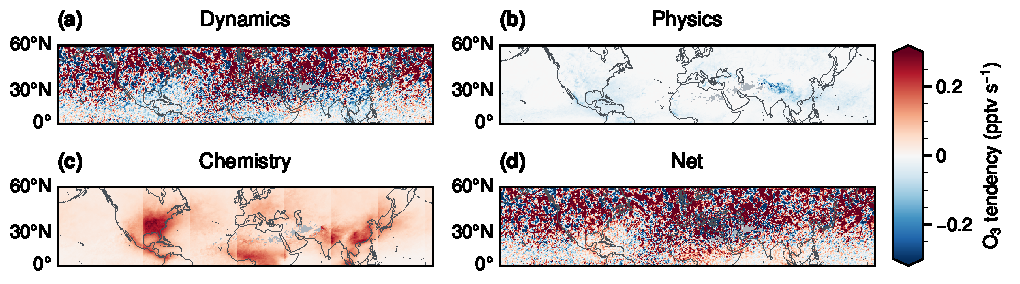
\includegraphics[width=15cm]{./figures/uto3_tendency.pdf}
    \caption{
    2019年6--8月北半球中低纬度MERRA2-GMI模拟的261 hPa高度O$_3$的平均趋势:
    (a)动力(b)物理(c)化学(d)净趋势。\\
    Figure \ref{fig:uto3_tendency}. The mean tendency of O$_3$ simulated by MERRA2-GMI at 261 hPa due to (a) dynamics, (b) physics, (c) chemistry, and (d) net tendency at the northern middle and low latitudes for June--August in 2019.
    }
    \label{fig:uto3_tendency}
\end{figure}


\begin{figure}[!htbp]
    \centering
    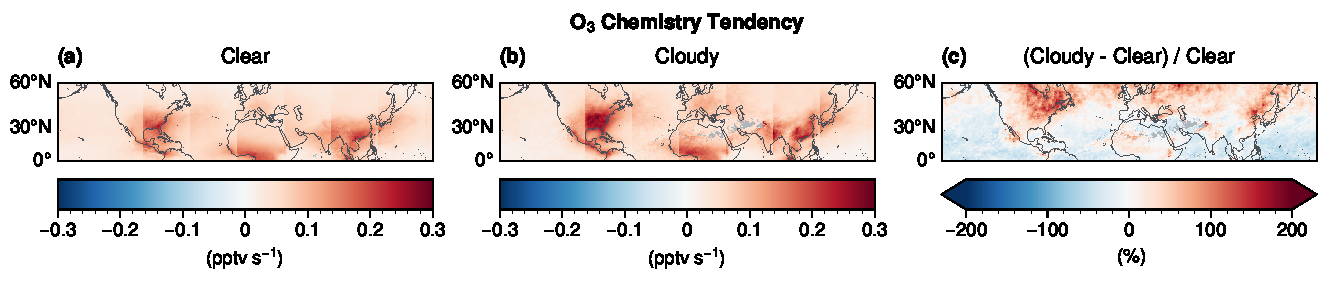
\includegraphics[width=15cm]{./figures/uto3_chem_tendency.pdf}
    \caption{
    2019年6--8月北半球中低纬度MERRA2-GMI模拟的261 hPa高度O$_3$的平均化学趋势:
    (a)晴空条件(b)有云条件(c)两者的相对差。\\
    Figure \ref{fig:uto3_chem_tendency}. The mean chemistry tendency of O$_3$ simulated by MERRA2-GMI for 261 hPa at the northern middle and low latitudes for June--August in 2019:
    (a) clear condition, (b) cloudy condition, (c) percentage differences.
    }
    \label{fig:uto3_chem_tendency}
\end{figure}


\subsection{闪电氮氧化物的影响} \label{sec:lnox_effects}

我们将开启和不开启LNO排放所得到的中国东南部O$_3$累计物理变化速率进行对比,从而得到LNO$_x$对O$_3$的影响(表1)。
在2019年个例的对流旺盛期和整个生命周期中,LNO$_x$使得O$_3$的净产量降低了25\%。
对于2020年个例,由于站点附近闪电密度较小,化学贡献导致的O$_3$浓度下降不显著($\leq$1\%)。
而前人研究表明,LNO$_x$在天的时间尺度范围内可提高下风向的O$_3$产量\citep{Pickering.1996,DeCaria.2005}。
因此,有必要准确估计LNO$_x$的产率(见第\ref{chapter:PE}章)。

\begin{table*}[h]
\centering
\caption{平均O$_3$累积趋势的过程分析(10--14 km)\\ Table \ref{table:ipr} Process analysis table for the mean O$_3$ integrated tendencies (10--14 km)}
\begin{tabular}{@{\extracolsep{\fill}} cccccc}
\hline
  Period           & Time             & LNO (mol/flash) & advh + advz$^*$       & chem$^*$              & net$^*$    \\
\hline
Life Cycle         & 2019-07-25       & 0               & -3.3 (-24.6 \%)        & 16.7 (124.6 \%)        & 13.4       \\
                   & (03:20--05:40)   & 500             & -2.3 (-28.8 \%)        & 10.3 (128.8 \%)        & 8.0        \\
\cline{2-6}
                   & 2020-09-01       & 0               & 3.4  (9.6 \%)          & 32.0 (90.4 \%)         & 35.4       \\
                   & (04:20--06:40)   & 500             & 4.4  (12.1 \%)         & 31.9 (87.8 \%)         & 36.3       \\
\hline
Convective Period   & 2019-07-25      & 0              & -19.6 (140.0 \%)       & 5.6 (-40.0 \%)         & -14.0      \\
                    & (04:20--05:00)  & 500            & -20.0 (114.3 \%)       & 2.5 (-14.3 \% )        & -17.5      \\
\cline{2-6}
                    & 2020-09-01      & 0              & -9.7  (-131.1 \%)      & 17.1 (231.1 \% )       & 7.4        \\
                    & (05:40--06:20)  & 500            & -10.1 (-148.5 \%)      & 16.9 (248.5 \% )       & 6.8        \\
\hline
\multicolumn{6}{l}{$^{*}$单位是 10$^{10}$ molec. cm$^{-3}$。百分比是每种贡献在净O$_3$变化中的比例。} \\
\multicolumn{6}{l}{$^{*}$The unit is 10$^{10}$ molec. cm$^{-3}$. The percentage is the proportion of each part in the net O$_3$ change.}
\end{tabular}
\label{table:ipr}
\end{table*}


此外,我们利用TROPOMI数据将对流分为三个区域:新生闪电区、闪电下风向和闪电老化区(详见第\ref{sec:lnox_affects_tropomi}节和图\ref{fig:china_s5p_amf_diff})。
首先使用基于不同LNO产率的模拟结果,获得O$_3$差异($\Delta$O$_3$) 的廓线(图\ref{fig:irr_timeseries}(a--c))。
$\Delta$O$_3$在2--5 km之间大部分为正(< 1 ppbv),在5--12 km 之间为负,
这与\citet{Ott.2007}研究的个例结论不一致,他们得出在所有高度上的臭氧都产生净损失(< 4 ppbv)。
此外,较高的LNO产率(700 mol/闪电)与默认产率(500 mol /闪电)所得的结果相比,所有高度的O$_3$浓度降低了不到 1 ppbv,甚至导致闪电下风向2--5 km之间的$\Delta$O$_3$为负(图\ref{fig:irr_timeseries}b)。
由于LNO$_x$在8--10 km 之间达到峰值,O$_3$浓度也在此层降低(2.6 ppbv)最多。

接着,我们应用积分反应速率(IRR)来评估O$_3$变化的化学机制以及LNO对$\Delta$O$_3$的影响。
我们分两层来看该影响,因为800--500 hPa上$\Delta$O$_3$为正,500--200 hPa上$\Delta$O$_3$为负。
对流层O$_3$主要由五个反应速率项控制\citep{Pickering.1990}:

\begin{eqnarray}
  \frac{d}{dt}[\mathrm{O_3}] & = & k_1[\mathrm{NO}][\mathrm{HO_2}] + \sum_{i}  k_i[\mathrm{NO}][\mathrm{R_iO_2}] \nonumber \\
                             && - k_3[\mathrm{H_2O}][\mathrm{O(^1D)}] - k_4[\mathrm{HO_2}][\mathrm{O_3}] - k_5[\mathrm{OH}][\mathrm{O_3}]
\end{eqnarray}

其中k$_i$是过氧自由基 (R$_i$O$_2$)与NO之间的反应速率系数。
每个反应对O$_3$贡献的时间序列如图\ref{fig:irr_timeseries}(d--i)所示。
总体而言,由于2019年个例的垂直运动更强(见第\ref{sec:convec_impacts}节),故积分反应速率的时间序列变化更大,且所选两层的O$_3$总净化学产量保持正值。
具体而言,NO和HO$_2$之间的反应始终占主导地位,而RO$_2$对NO的氧化约占该产量的40\%--60\%。
O$_3$的主要损耗是光解反应(O(1D)和H$_2$O的反应),而O$_3$和OH之间的反应在对流期间与之相当。
O$_3$损耗的最低贡献,O$_3$ + HO$_2$ $\,\to\,$ OH + 2O$_2$,在对流旺盛期减少,因为LNO的产生捕获了本应与O$_3$反应的HO$_2$。
虽然LNO$_x$引起的总积分反应速率增加,在低层和高层分别为1.36$\times$10$^7$和2.60$\times$10$^6$ molec cm$^{-3}$ s$^{-1}$。
但是由于动力传输和与LNO$_x$化学贡献的综合作用,高层的O$_3$净产量实际上减少了(图\ref{fig:irr_timeseries}(a--c))。


\begin{figure}[h]
    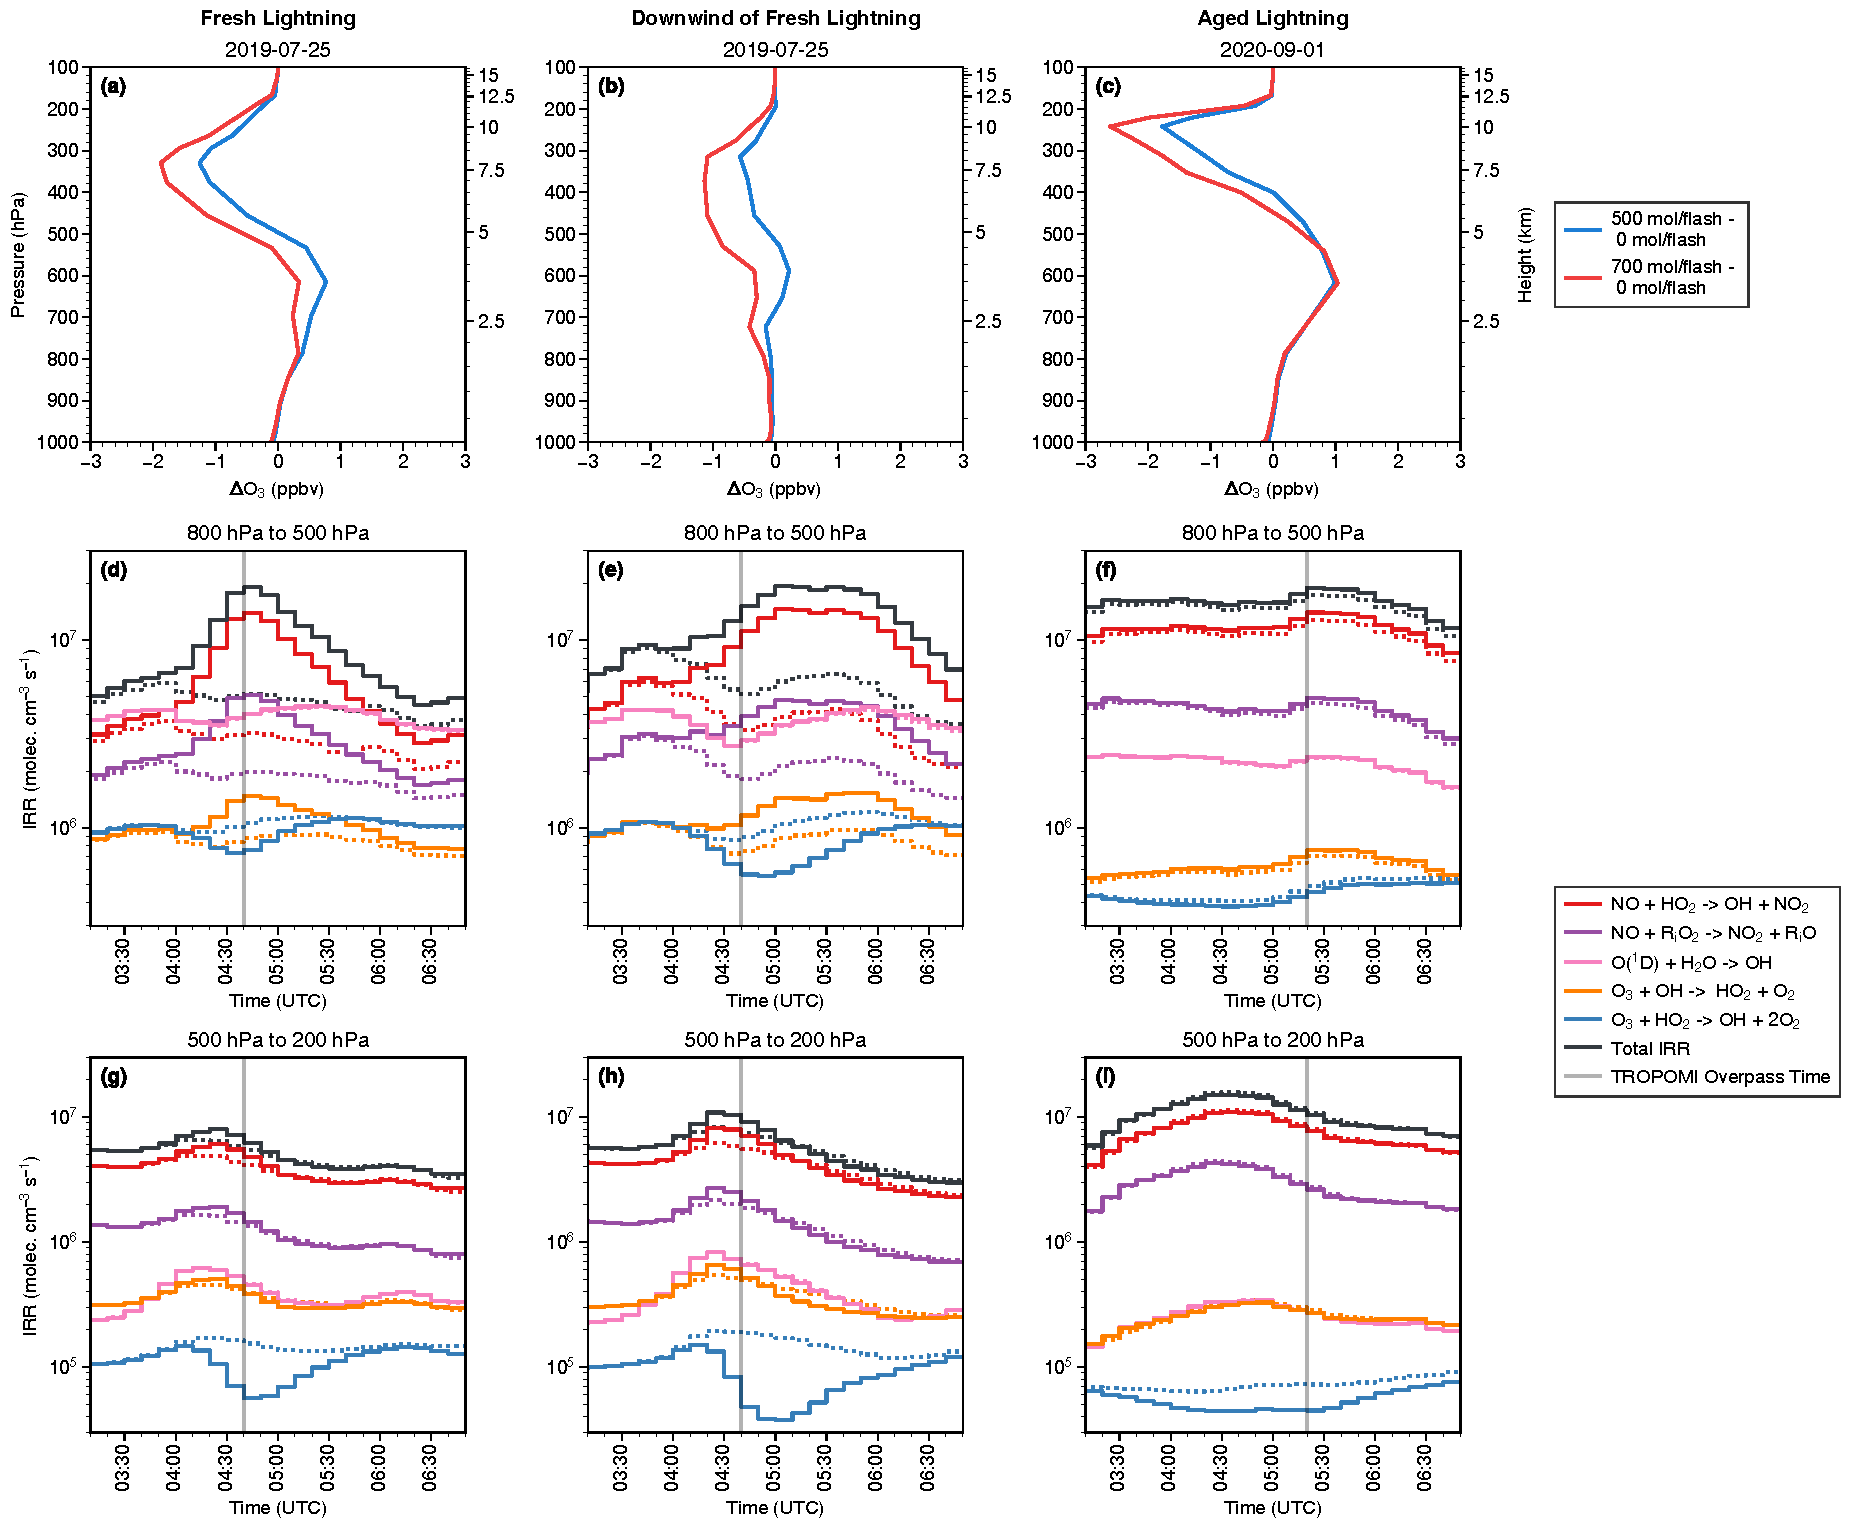
\includegraphics[width=16cm]{./figures/irr_timeseries.pdf}
    \caption{
    (a--c) 在图\ref{fig:china_s5p_amf_diff}定义的三个区域(新生闪电区、闪电下风向和闪电老化区)中,TROPOMI过境时由LNO$_x$所引起的O$_3$剖面变化。
    (d--f) 800 hPa 和 500 hPa 之间平均累积反应速率 (IRR) 的时间序列。其中图例显示了详细的物种和反应。总IRR是从生成O$_3$的IRR(红线和紫线)中减去O$_3$损失的IRR。
     实线为模拟中开启LNO (500 mol/flash)排放的IRR,而虚线表示没有LNO。
    (g--i) 与 (d--f) 相同,但在 500 hPa 和 200 hPa 之间。\\
    Figure \ref{fig:irr_timeseries}. (a--c) Changes in O$_3$ profiles due to LNO$_x$ at TROPOMI overpass time in three regions (fresh lightning region, downwind of fresh lightning, and aged lightning area) as defined in Fig. \ref{fig:china_s5p_amf_diff}.
    (d--f) Time series of the mean integrated reaction rate (IRR) between 800 hPa and 500 hPa.
    The legend shows detailed species and reactions.
    The Total IRR is the O$_3$ loss IRR subtracted from the O$_3$ production IRR (red and purple lines).
    The solid line shows the IRR with LNO (500 mol/flash) while the dashed line is without LNO.
    (g--i) Same as (d--f) but between 500 hPa and 200 hPa.
    }
    \label{fig:irr_timeseries}
\end{figure}

\section{本章小结}


本章不仅将云切片的O$_3$平均浓度和MLS O$_3$廓线与MERRA2-GMI模拟结果进行对比分析,
而且将中国东南部对流个例的探空试验与WRF-Chem模式结果相结合,对O$_3$垂直分布变化的贡献项进行了详细讨论;
主要结论如下:

\begin{enumerate}[label=(\arabic*), labelindent=\parindent, leftmargin=0pt, widest=0, itemindent=*, topsep=0pt, partopsep=0pt, parsep=0pt]

\item 在低纬地区,TROPOMI、MLS和MERRA2-GMI均显示上对流层的低O$_3$事件常发生于热带西太平洋,
而非洲中部由于对流输送的边界层高O$_3$浓度气团,上对流层O$_3$在有云条件下浓度更高;

\item 在中纬地区,TROPOMI的云切片结果较少,MLS和MERRA2-GMI的上对流层O$_3$趋势相反:
MERRA2-GMI模拟显示上对流层O$_3$浓度在有云时比晴空时浓度更低,MLS观测表明有云时上对流层O$_3$浓度增大,
鉴于MERRA2-GMI与TROPOMI的相近,我们将MLS在261 hPa高度层高估的O$_3$浓度归因于平流层过度的外推;

\item MERRA2-GMI在闪电频发的美国东南部的模拟结果显示,330--450 hPa高度不存在TROPOMI观测到的O$_3$峰值,
故MERRA2-GMI模拟中上对流层LNO$_2$的差异导致了O$_3$浓度的低估;

\item 闪电同化后的WRF-Chem对流模拟结果与观测相符,虽然WRF-Chem模式结果倾向于低估O$_3$浓度,
但其再现了O$_3$探空观测到的垂直分布结构及变化,即对流发生后上对流层的O$_3$和Q$_v$均增大;

\item MERRA2-GMI和WRF-Chem的O$_3$趋势分析结果表明,虽然动力输送项在对流旺盛期间占主导,
但在污染地区化学反应的正贡献在整个生命期更为重要。

\item 中国东南部的对流个例模拟显示,虽然LNO$_x$使得累积净化学反应速率增大,
但动力输送和化学反应的综合作用降低了上对流层O$_3$浓度。

\end{enumerate}
